%********************************************************************
% Appendix
%*******************************************************
% If problems with the headers: get headings in appendix etc. right
%\markboth{\spacedlowsmallcaps{Appendix}}{\spacedlowsmallcaps{Appendix}}
\chapter{Ejemplo completo de una medición}\label{ch:appendixSampleScanImages}

%\section{Framework para adquisición de imágenes}

%\section{Framework para calibración de cámaras}

%\section{Subpixel resolution para esquinas patrón calibración}

%\section{Post procesamiento}

%\subsection{Filtrado}
%\subsubsection{Subsampling}
%\subsubsection{Moving least squares}

%\subsection{Reconstrucción de la superficie}


En la \autoref{fig:ejemploMedicionNubeDePuntos} se puede observar la nube de puntos obtenida como resultado de una medición. El color corresponde a la intensidad de cada punto, utilizando un mapa de color para hacer más clara su visualización. 

\begin{figure}[!bth]
    \myfloatalign
        \subfloat{
            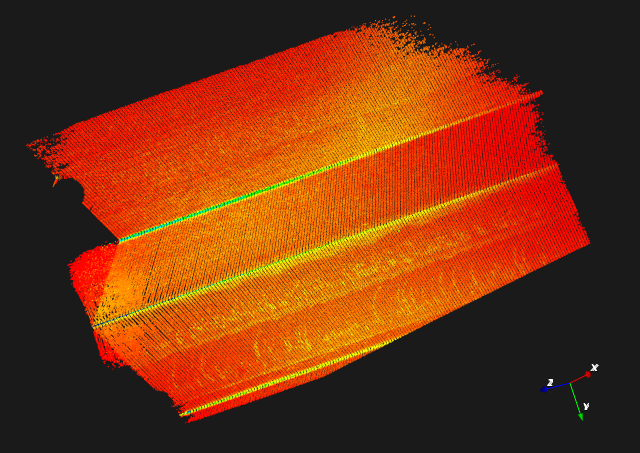
\includegraphics[width=0.49\linewidth]{images/soft/render3dView1}
        }
        \subfloat{
            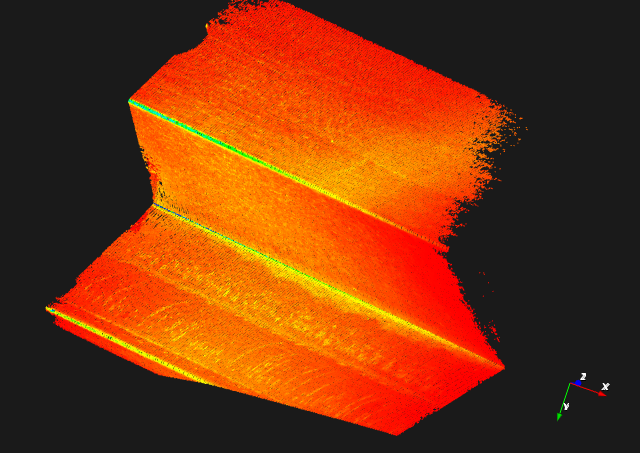
\includegraphics[width=0.49\linewidth]{images/soft/render3dView2}
        }
        \caption{Ejemplo de una medición: nube de puntos}
        \label{fig:ejemploMedicionNubeDePuntos}
\end{figure}

En la \autoref{fig:ejemploMedicionSuperficie} se muestra la misma medición pero luego del post-procesamiento y con la superficie reconstruída utilizando triángulos. En este caso no mantenemos el color (la intensidad) de cada punto, ya que utilizamos un modelo simple de iluminación para que se puedan observar de mejor manera las variaciones en la superficie.

\begin{figure}[!bth]
    \myfloatalign
        \subfloat{
            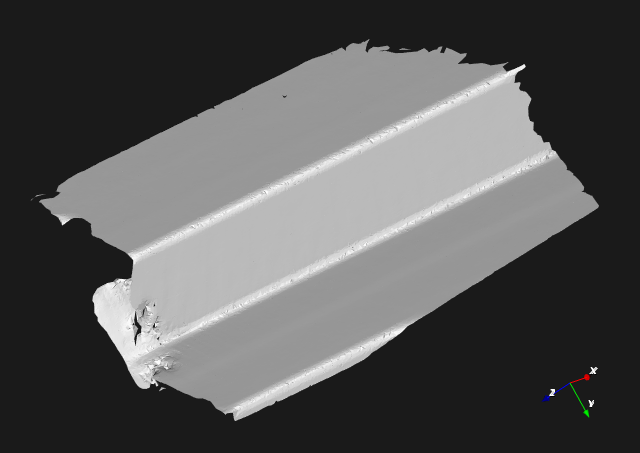
\includegraphics[width=0.49\linewidth]{images/soft/render3dViewSurface1}
        }
        \subfloat{
            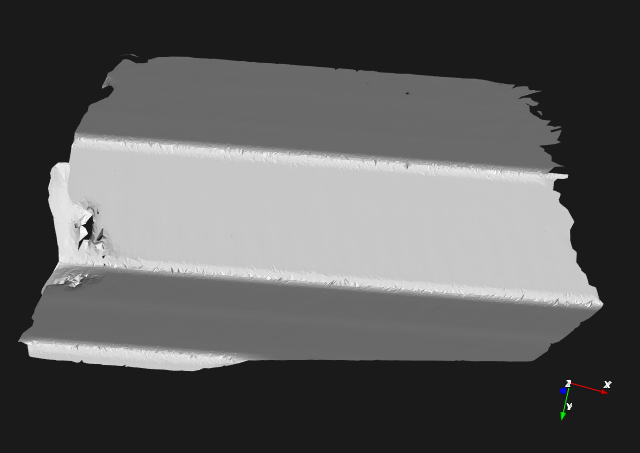
\includegraphics[width=0.49\linewidth]{images/soft/render3dViewSurface2}
        }
        \caption{Ejemplo de una medición: superficie reconstruída}
        \label{fig:ejemploMedicionSuperficie}
\end{figure}

A continuación se muestra el conjunto completo de imagenes utilizados para obtener la medición. 
%En las figuras \ref{fig:ejemploProyeccionCamaraIzquierda0a4} y \ref{fig:ejemploProyeccionCamaraIzquierda5a9} se muestran las correspondientes a la cámara izquierda mientras que en las figuras \ref{fig:ejemploProyeccionCamaraDerecha0a4} y \ref{fig:ejemploProyeccionCamaraDerecha5a9} se muestras las correspondientes a la cámara derecha.

% En las figuras \ref{fig:ejemploProyeccionCamaraIzquierda0a4} y \ref{fig:ejemploProyeccionCamaraIzquierda5a9} se muestra el conjunto de imagenes correspondientes a la cámara izquierda utilizado para obtener la medición. En las figuras \ref{fig:ejemploProyeccionCamaraDerecha0a4} y \ref{fig:ejemploProyeccionCamaraDerecha5a9} se muestras las correspondientes a la cámara derecha.

\begin{figure}[!h!]
    \myfloatalign
        \subfloat{
            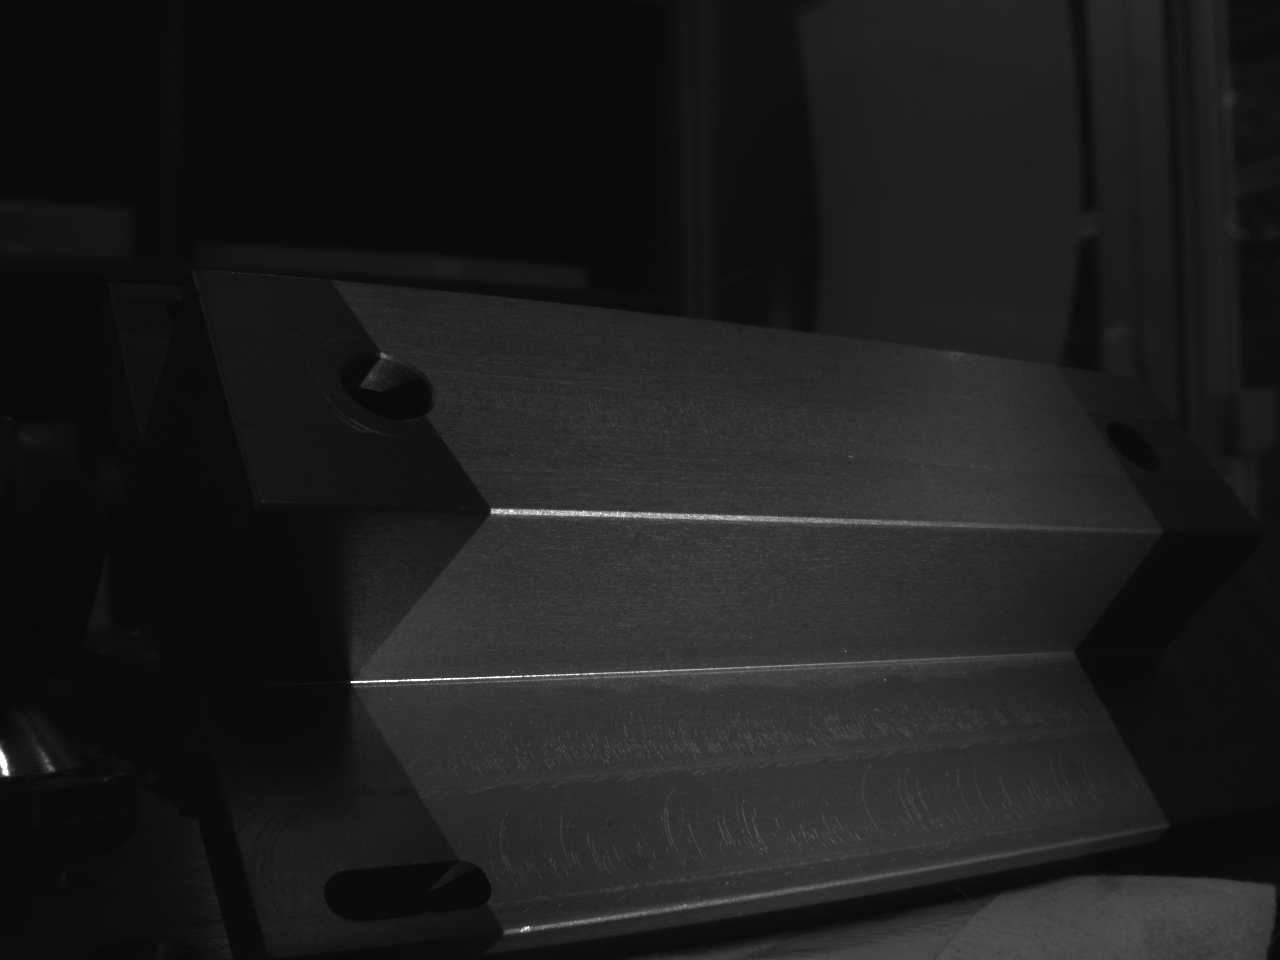
\includegraphics[width=0.49\linewidth]{images/snapshots_scan/SIMULATED-LEFT-LUMENERA-SN8010129/gray_00}
        }
        \subfloat{
            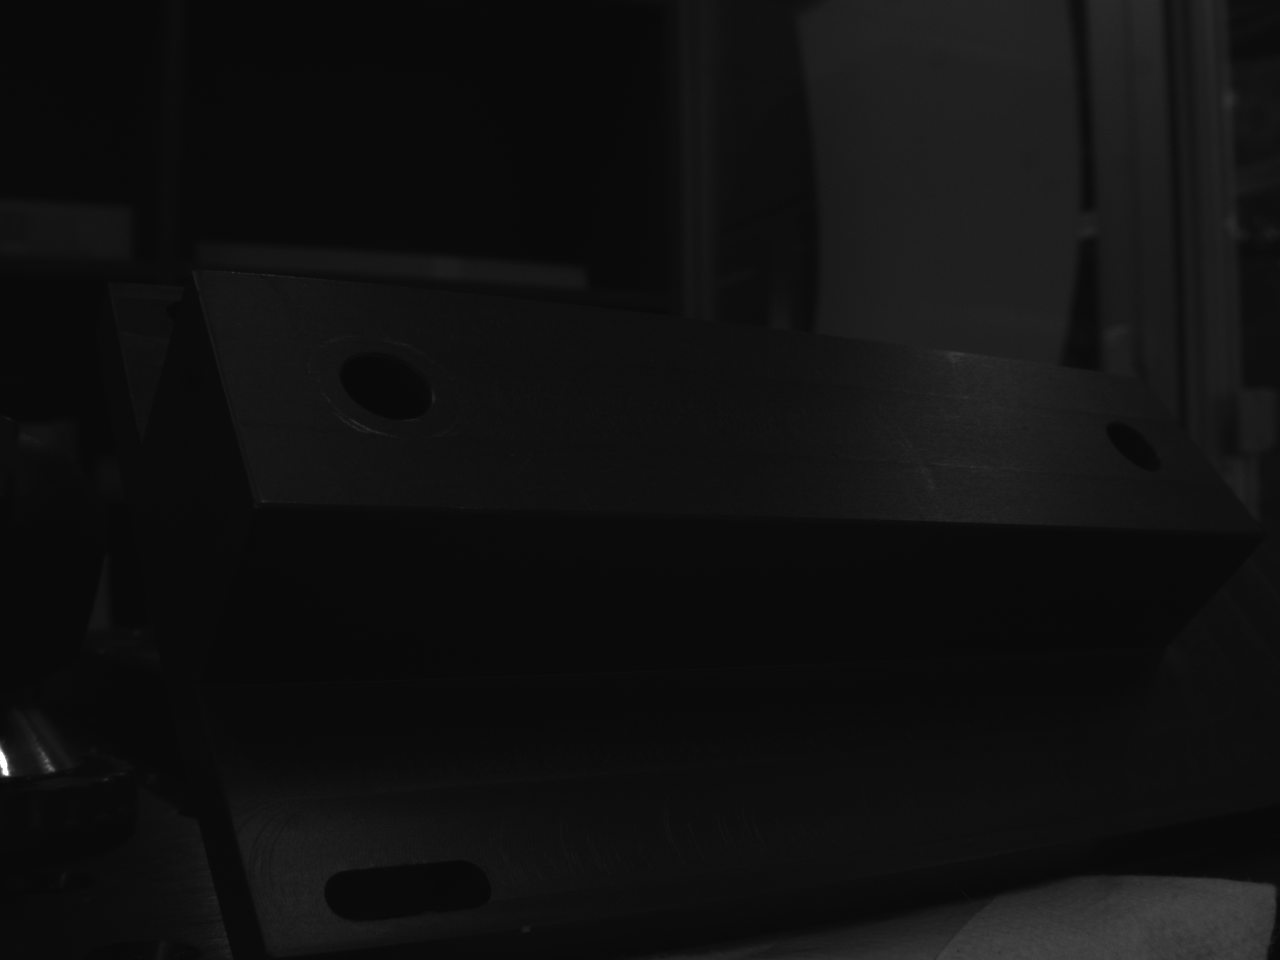
\includegraphics[width=0.49\linewidth]{images/snapshots_scan/SIMULATED-LEFT-LUMENERA-SN8010129/gray_00_inv}
        }
        \\
        \subfloat{
            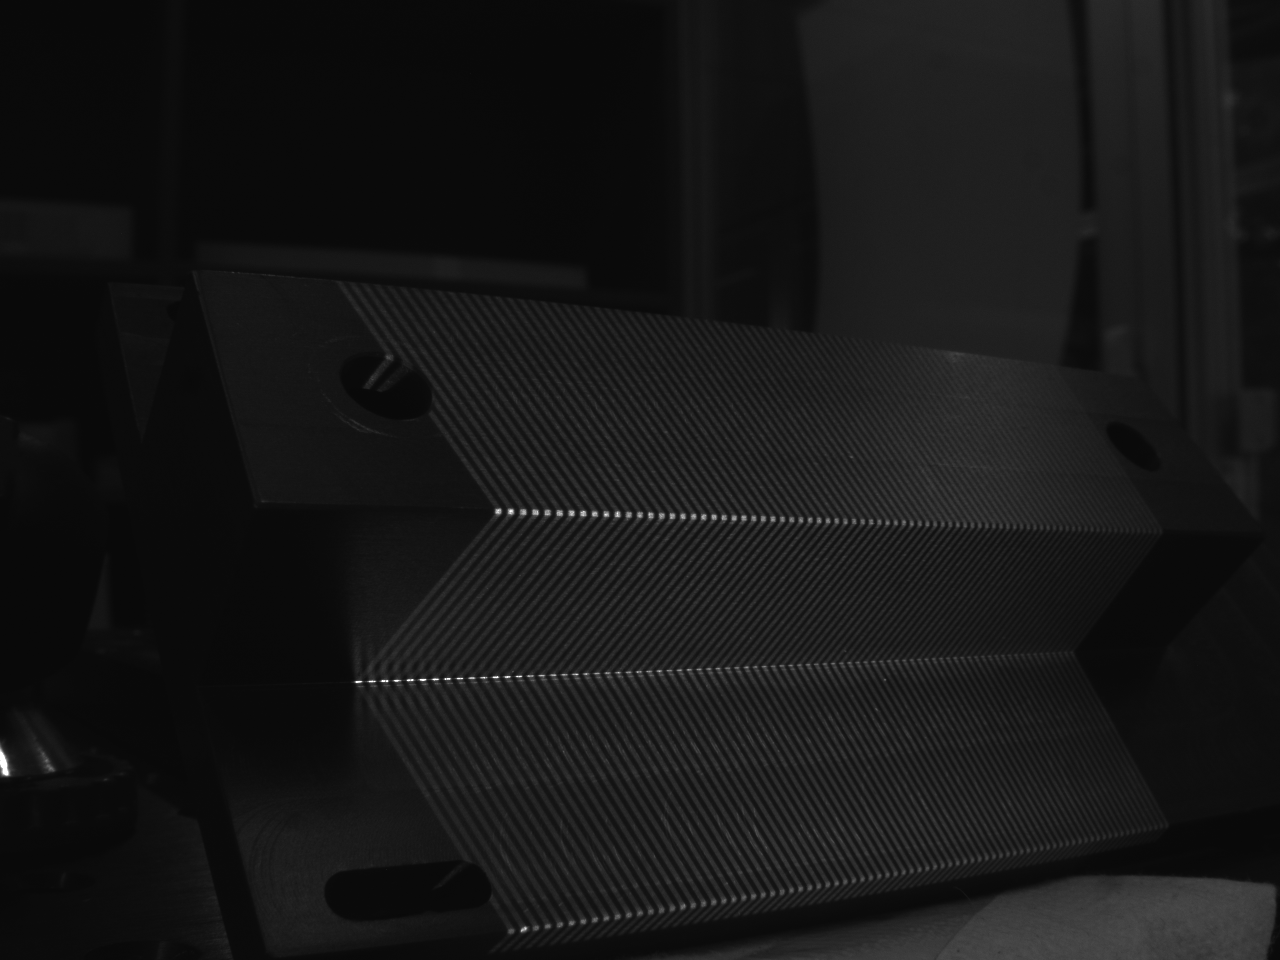
\includegraphics[width=0.49\linewidth]{images/snapshots_scan/SIMULATED-LEFT-LUMENERA-SN8010129/gray_01}
        }
        \subfloat{
            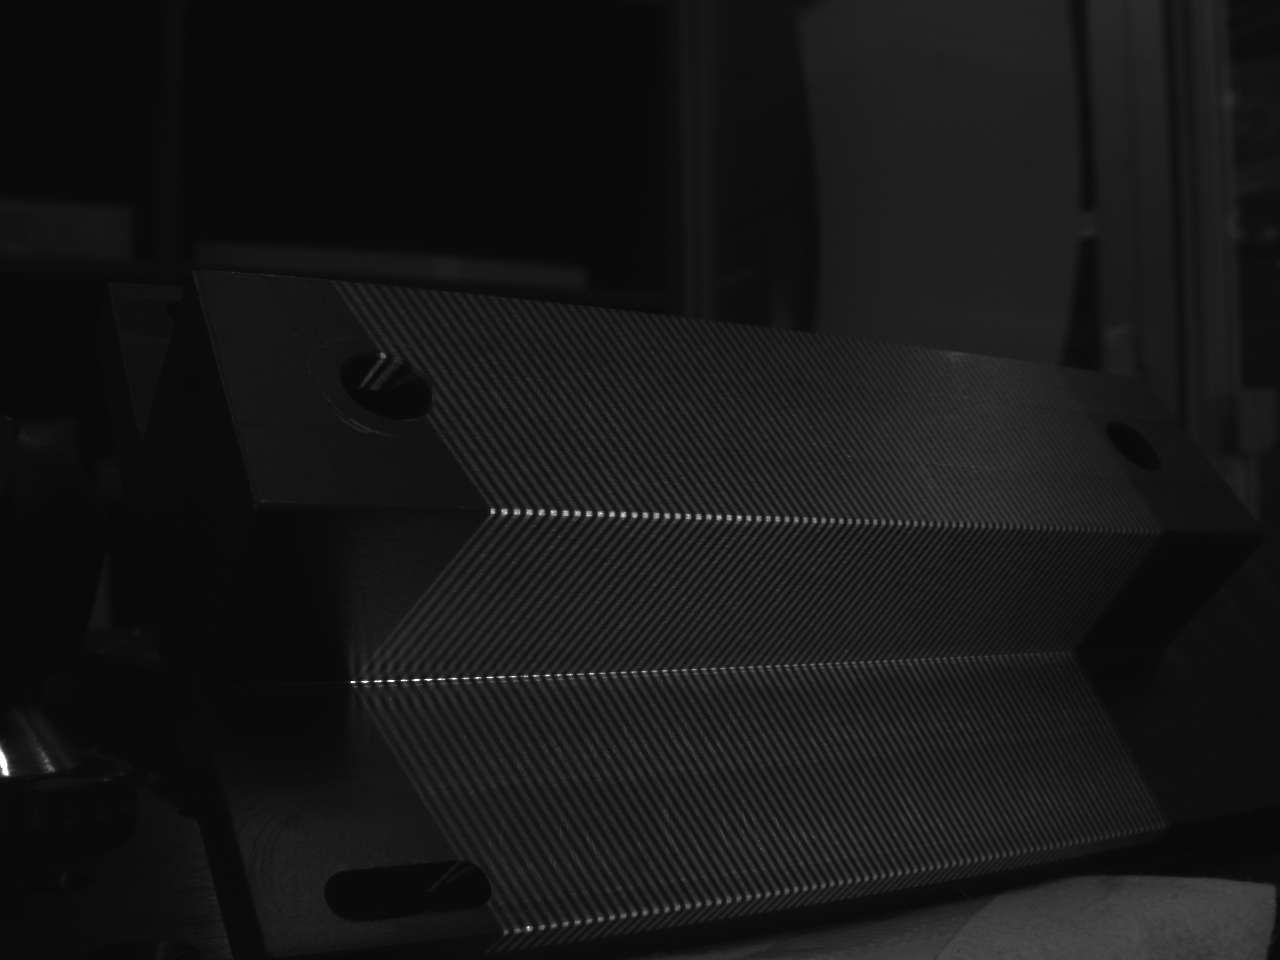
\includegraphics[width=0.49\linewidth]{images/snapshots_scan/SIMULATED-LEFT-LUMENERA-SN8010129/gray_01_inv}
        }
        \\
        \subfloat{
            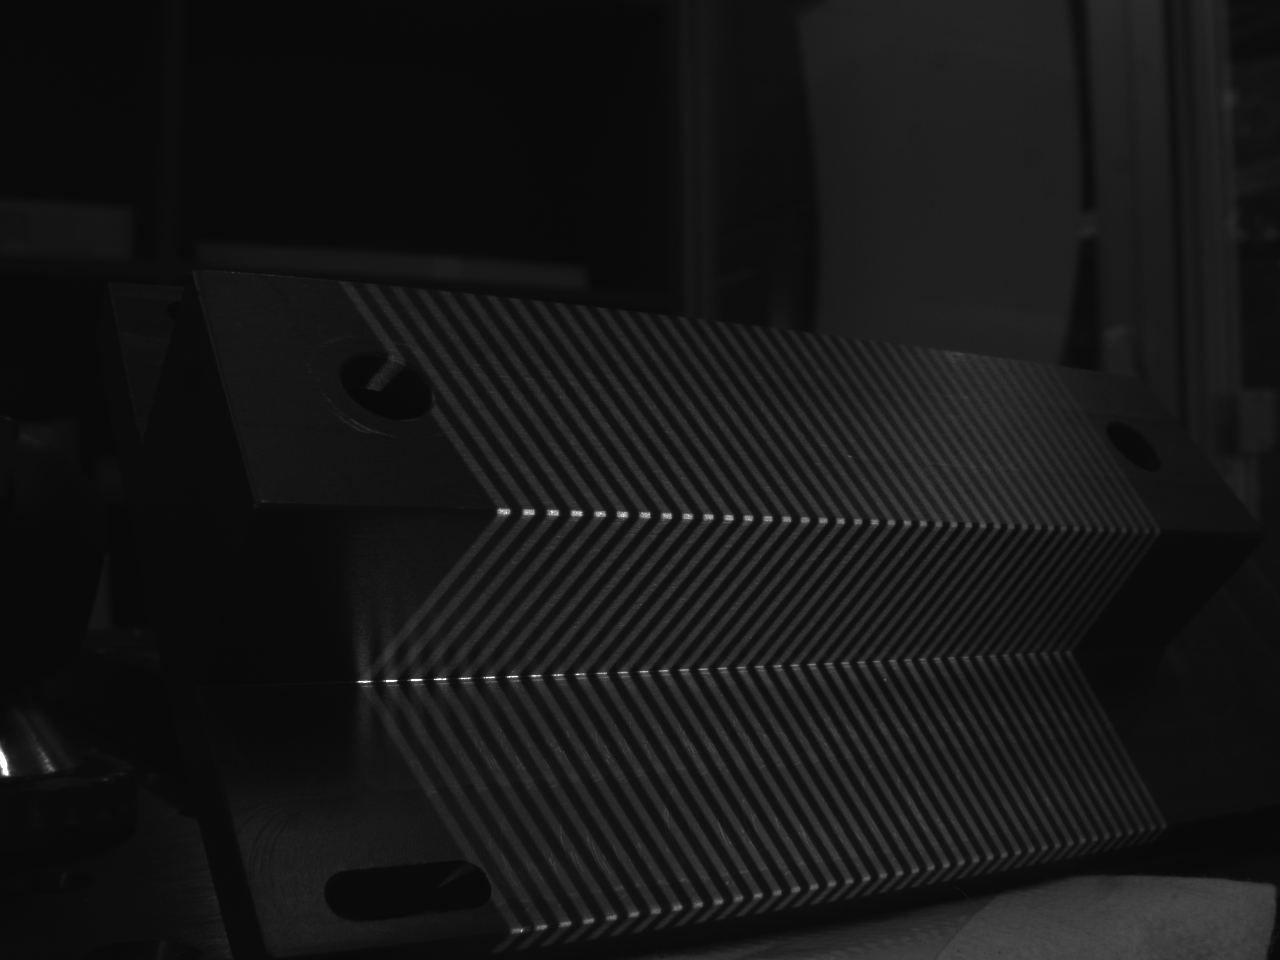
\includegraphics[width=0.49\linewidth]{images/snapshots_scan/SIMULATED-LEFT-LUMENERA-SN8010129/gray_02}
        }
        \subfloat{
            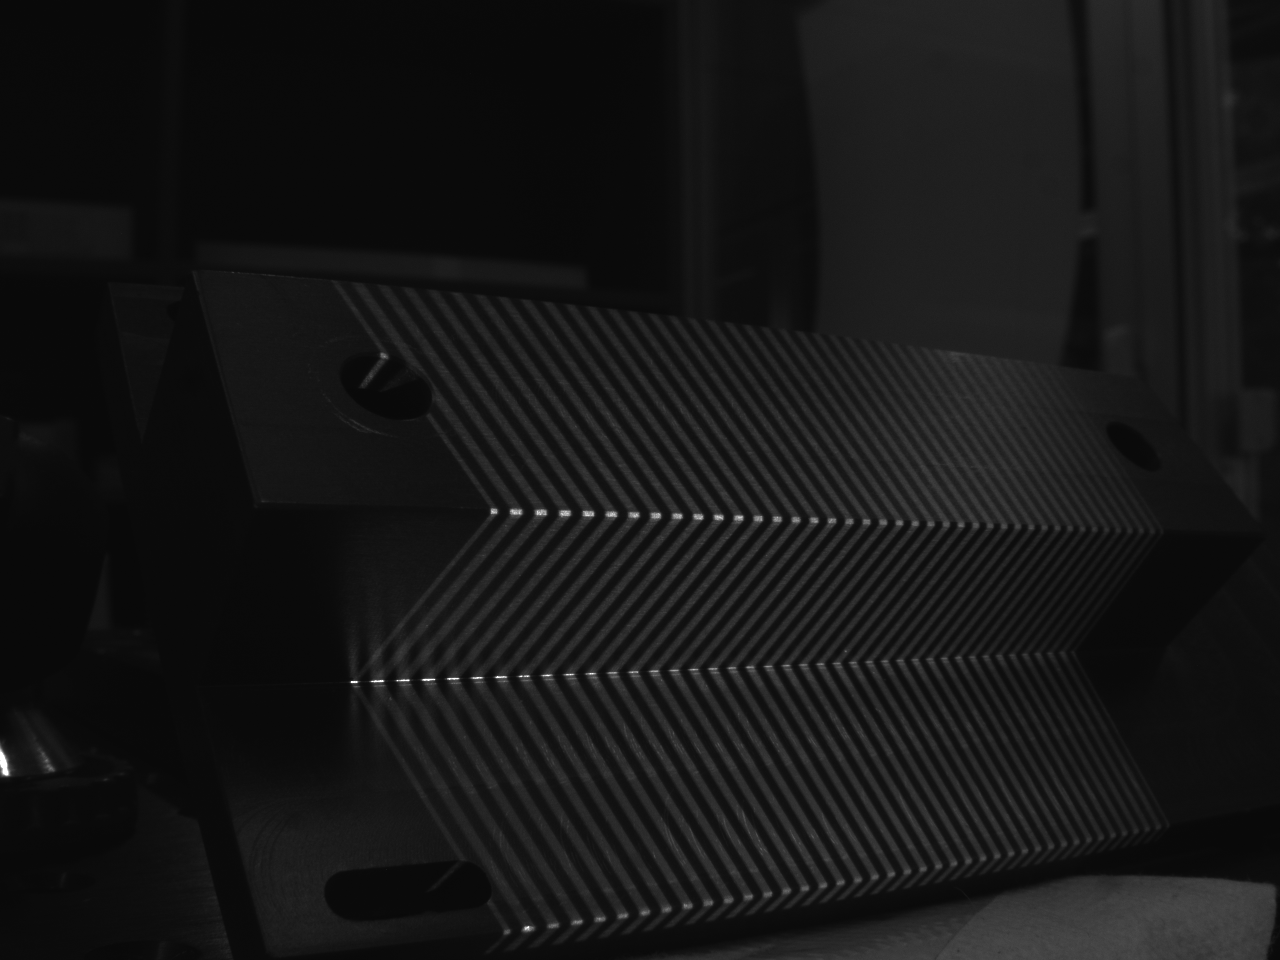
\includegraphics[width=0.49\linewidth]{images/snapshots_scan/SIMULATED-LEFT-LUMENERA-SN8010129/gray_02_inv}
        }
        \\
        \subfloat{
            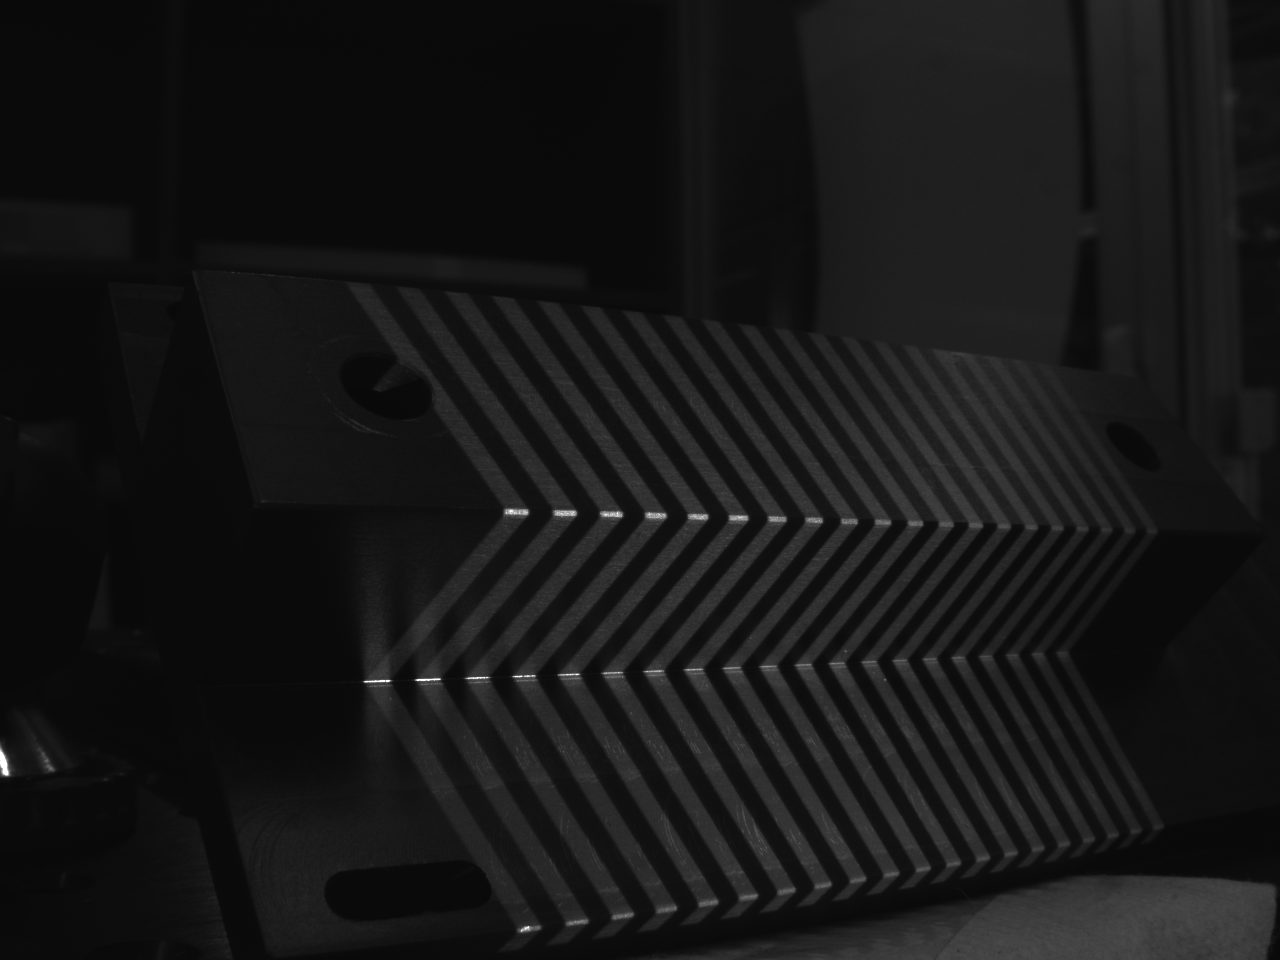
\includegraphics[width=0.49\linewidth]{images/snapshots_scan/SIMULATED-LEFT-LUMENERA-SN8010129/gray_03}
        }
        \subfloat{
            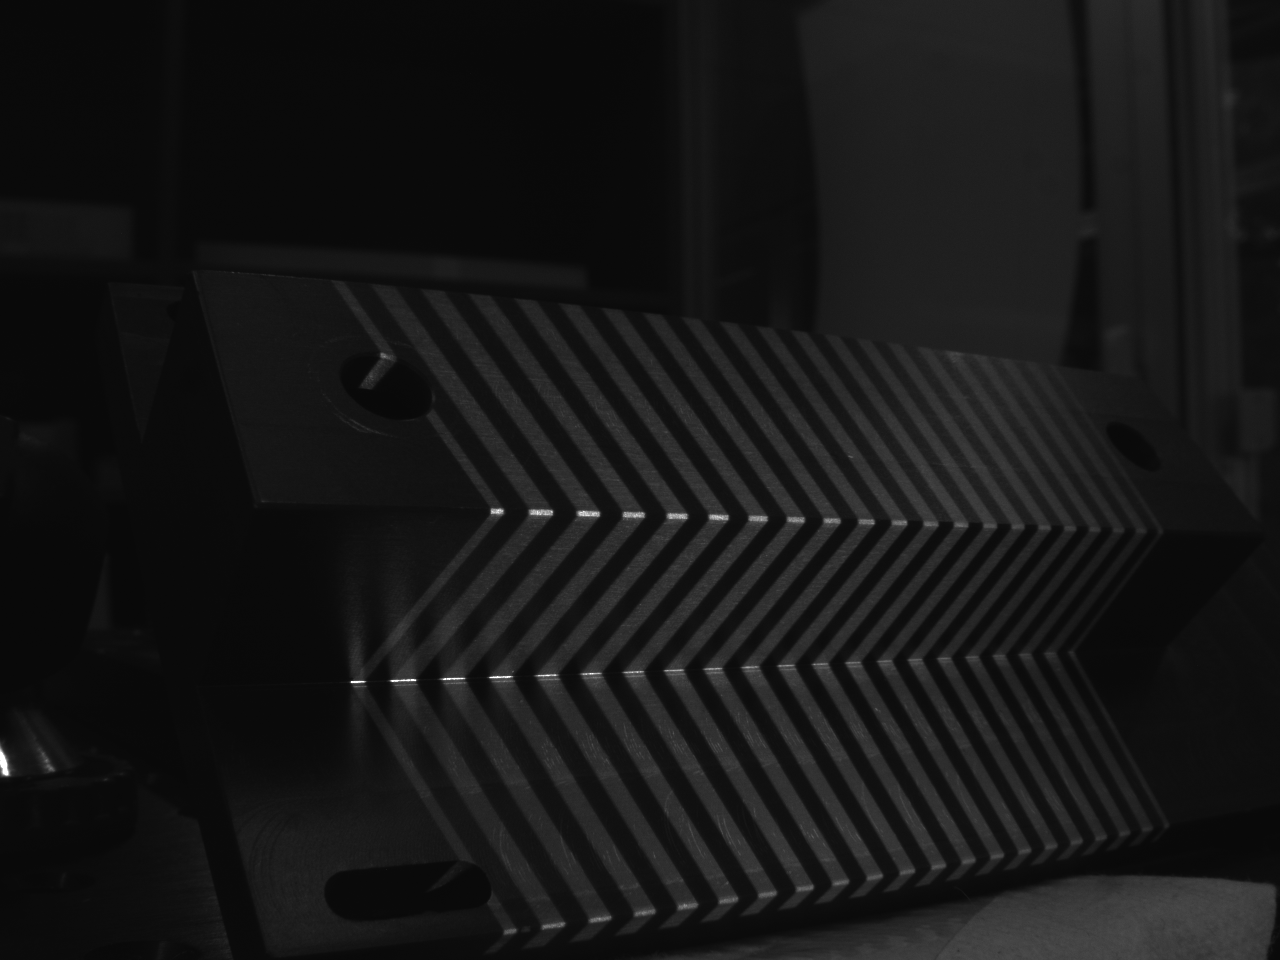
\includegraphics[width=0.49\linewidth]{images/snapshots_scan/SIMULATED-LEFT-LUMENERA-SN8010129/gray_03_inv}
        }
        \\
        \subfloat{
            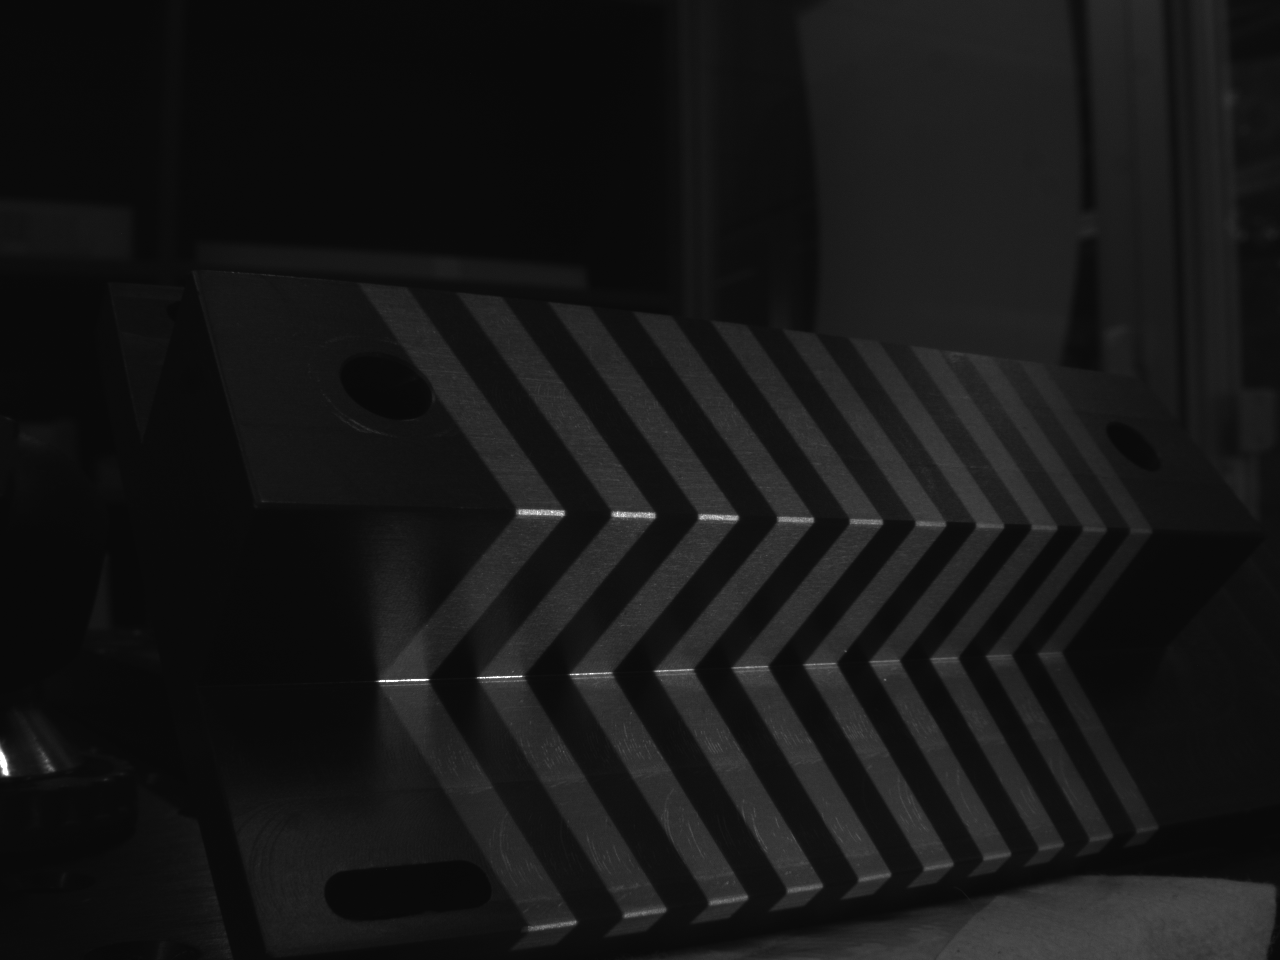
\includegraphics[width=0.49\linewidth]{images/snapshots_scan/SIMULATED-LEFT-LUMENERA-SN8010129/gray_04}
        }
        \subfloat{
            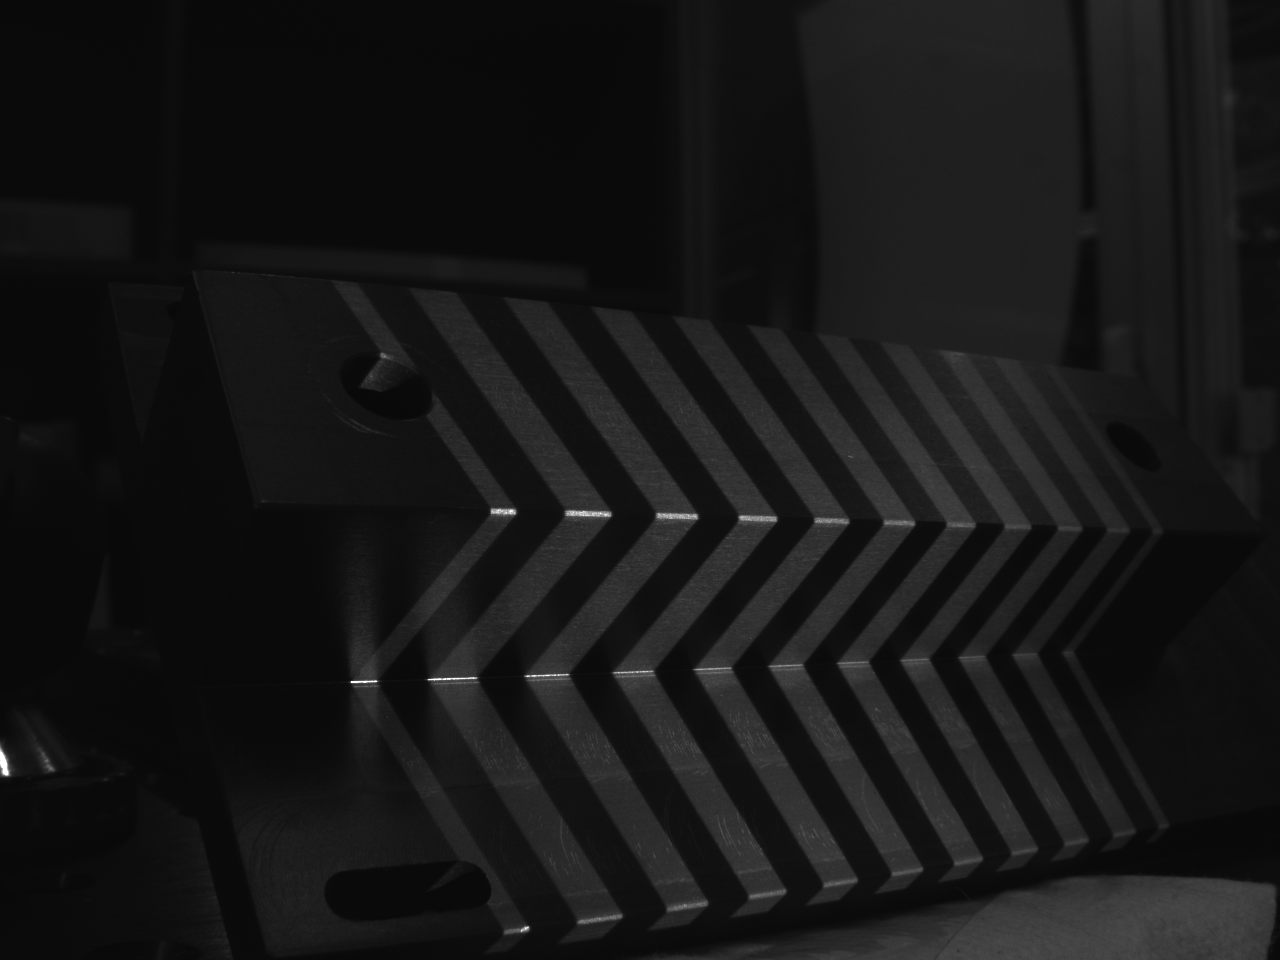
\includegraphics[width=0.49\linewidth]{images/snapshots_scan/SIMULATED-LEFT-LUMENERA-SN8010129/gray_04_inv}
        }
        \caption{Cámara izquierda: 5 primeros patrones proyectados (izq.) y su inverso (der.)}
        \label{fig:ejemploProyeccionCamaraIzquierda0a4}
\end{figure}

\begin{figure}[!h!]
    \myfloatalign
        \subfloat{
            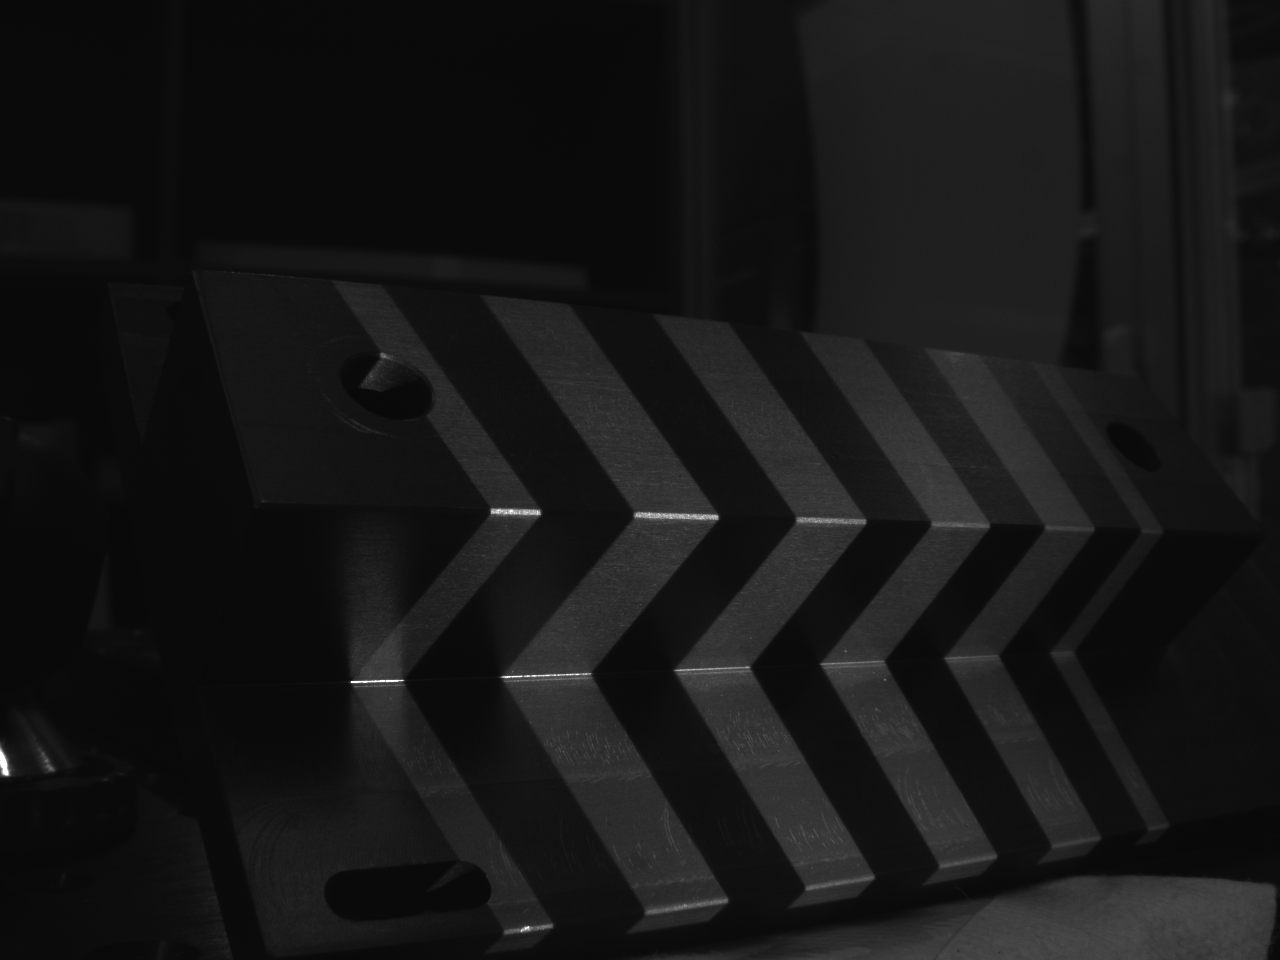
\includegraphics[width=0.49\linewidth]{images/snapshots_scan/SIMULATED-LEFT-LUMENERA-SN8010129/gray_05}
        }
        \subfloat{
            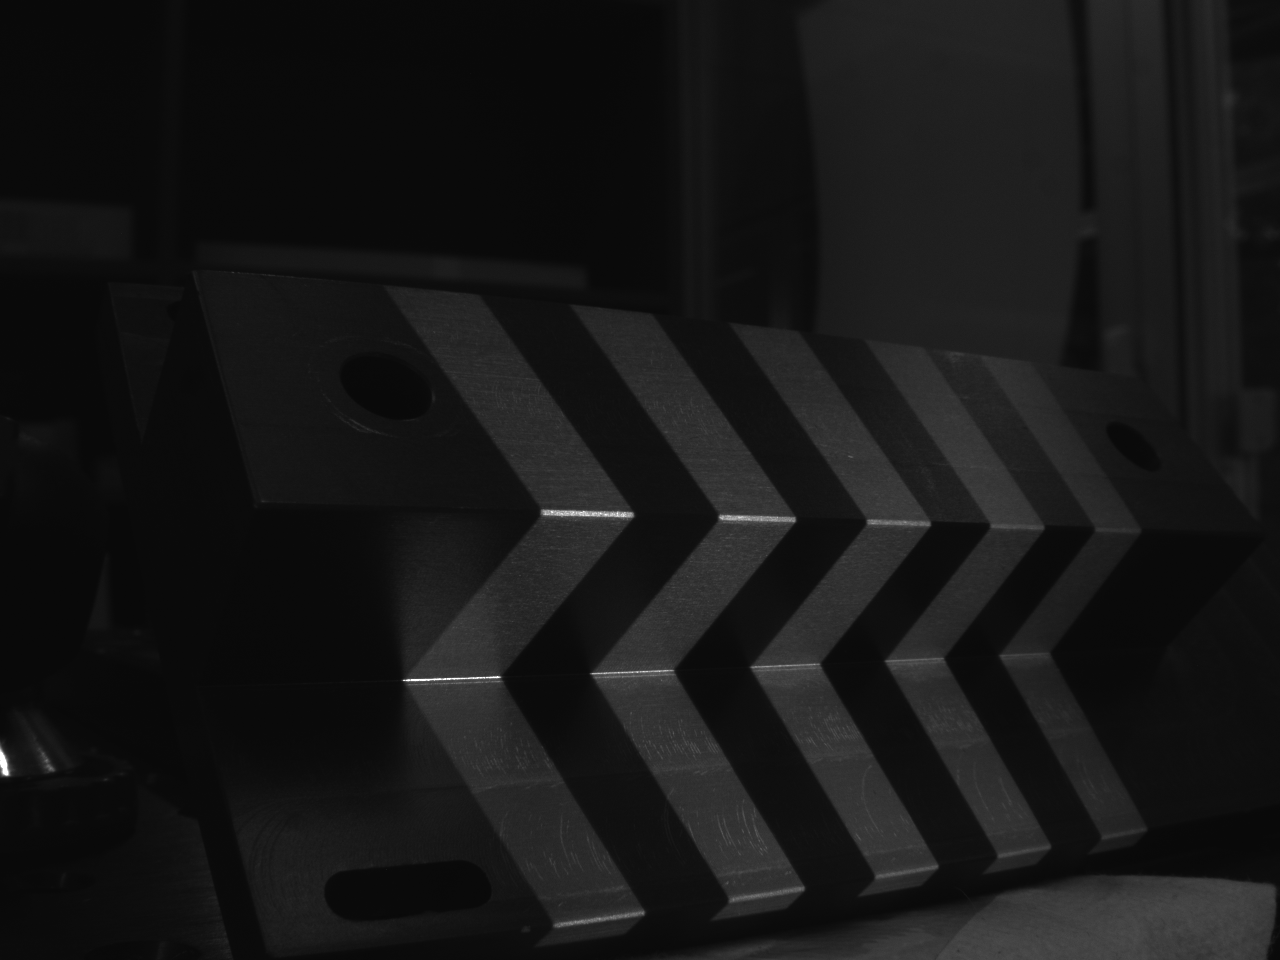
\includegraphics[width=0.49\linewidth]{images/snapshots_scan/SIMULATED-LEFT-LUMENERA-SN8010129/gray_05_inv}
        }
        \\
        \subfloat{
            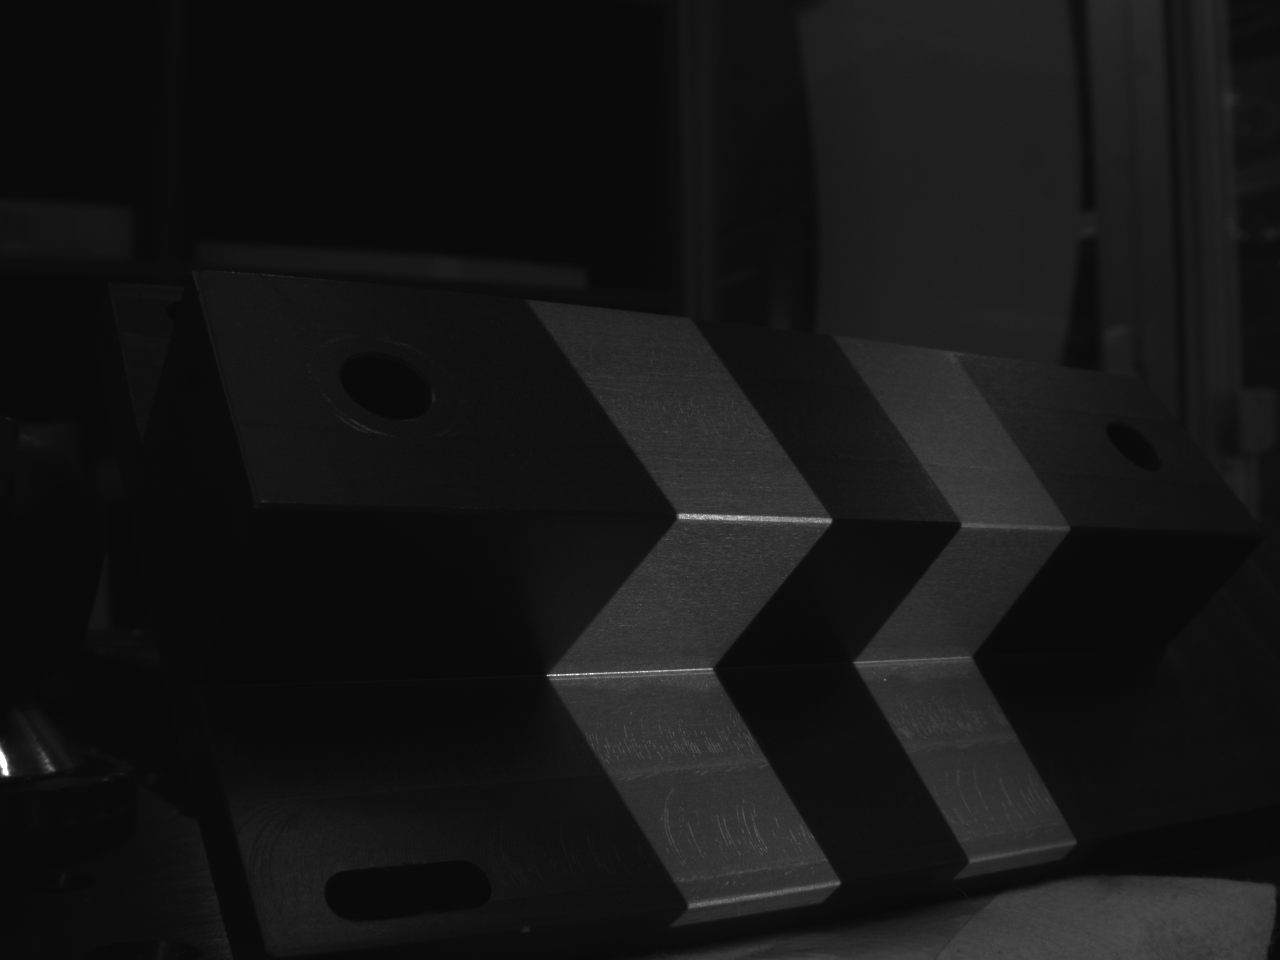
\includegraphics[width=0.49\linewidth]{images/snapshots_scan/SIMULATED-LEFT-LUMENERA-SN8010129/gray_06}
        }
        \subfloat{
            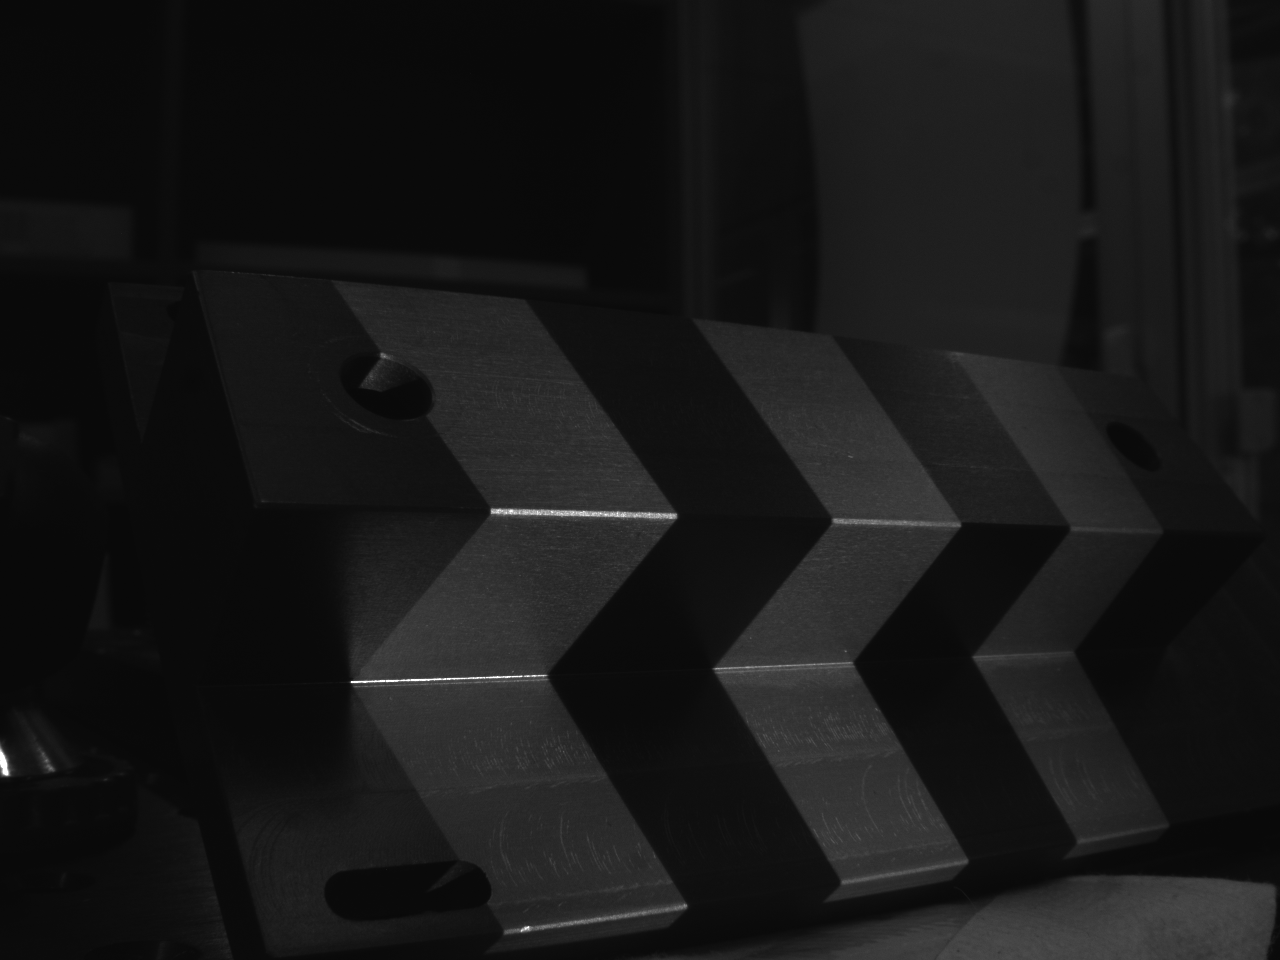
\includegraphics[width=0.49\linewidth]{images/snapshots_scan/SIMULATED-LEFT-LUMENERA-SN8010129/gray_06_inv}
        }
        \\
        \subfloat{
            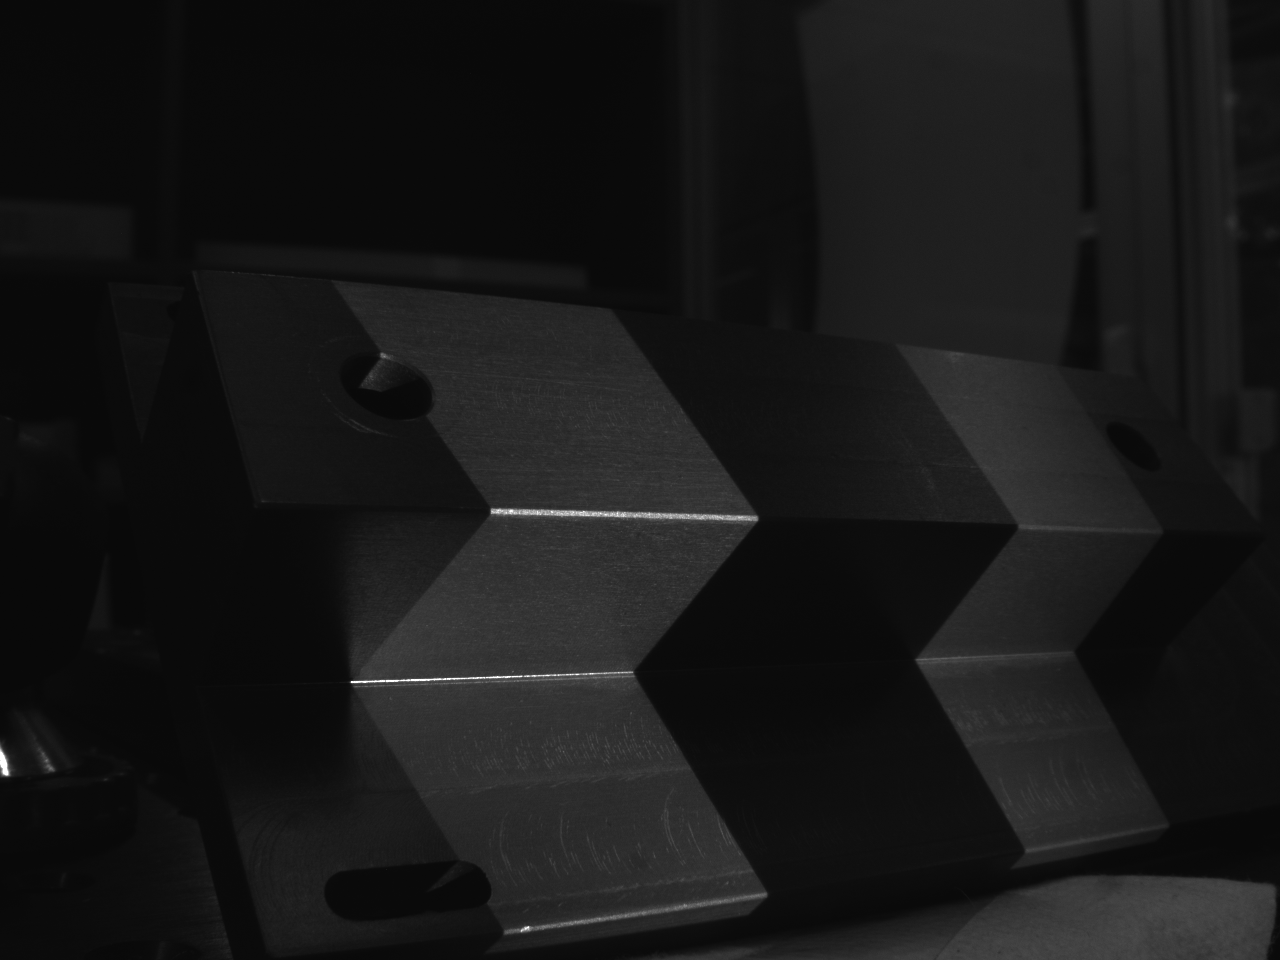
\includegraphics[width=0.49\linewidth]{images/snapshots_scan/SIMULATED-LEFT-LUMENERA-SN8010129/gray_07}
        }
        \subfloat{
            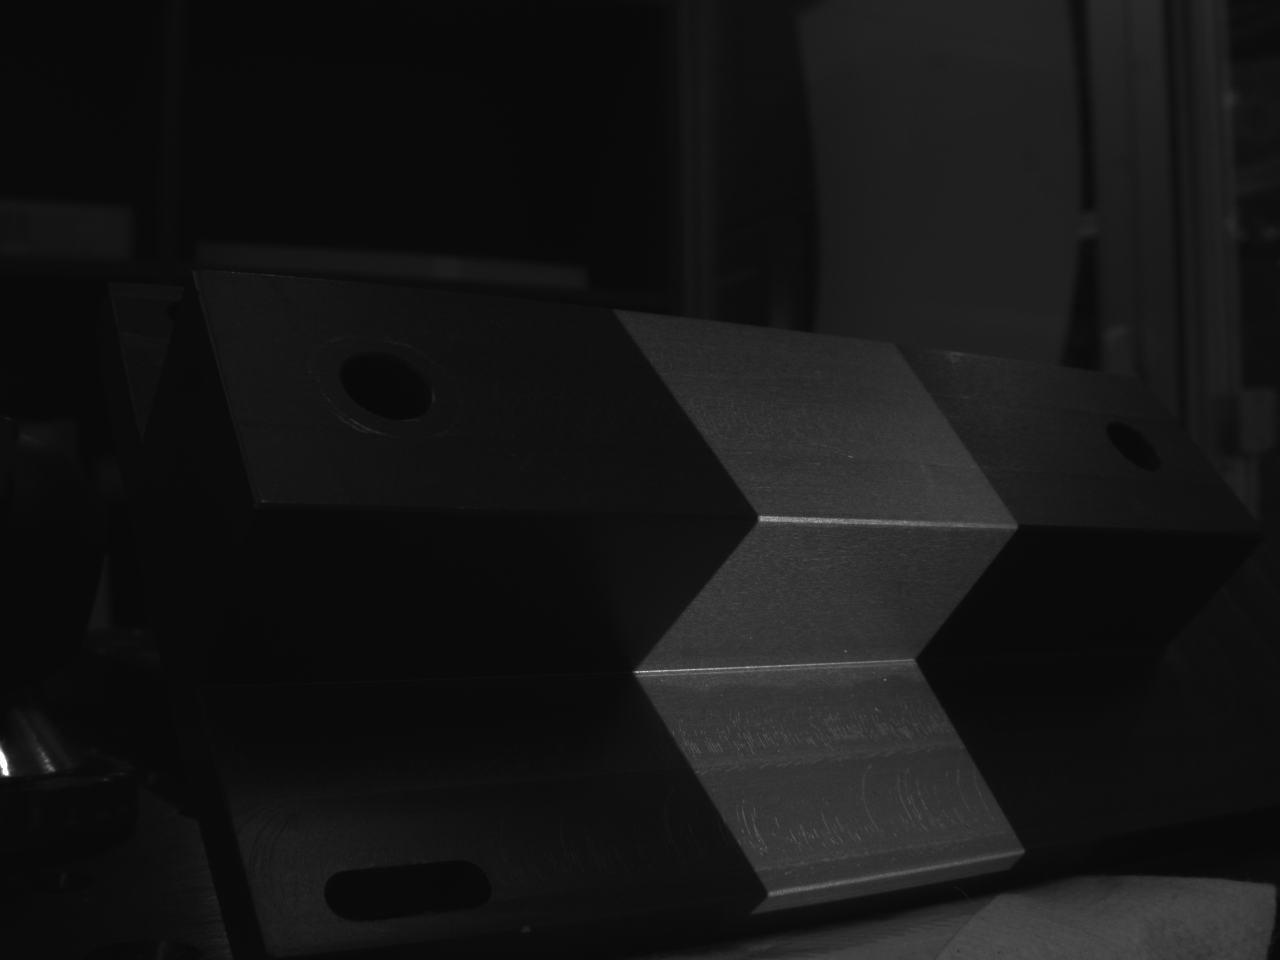
\includegraphics[width=0.49\linewidth]{images/snapshots_scan/SIMULATED-LEFT-LUMENERA-SN8010129/gray_07_inv}
        }
        \\
        \subfloat{
            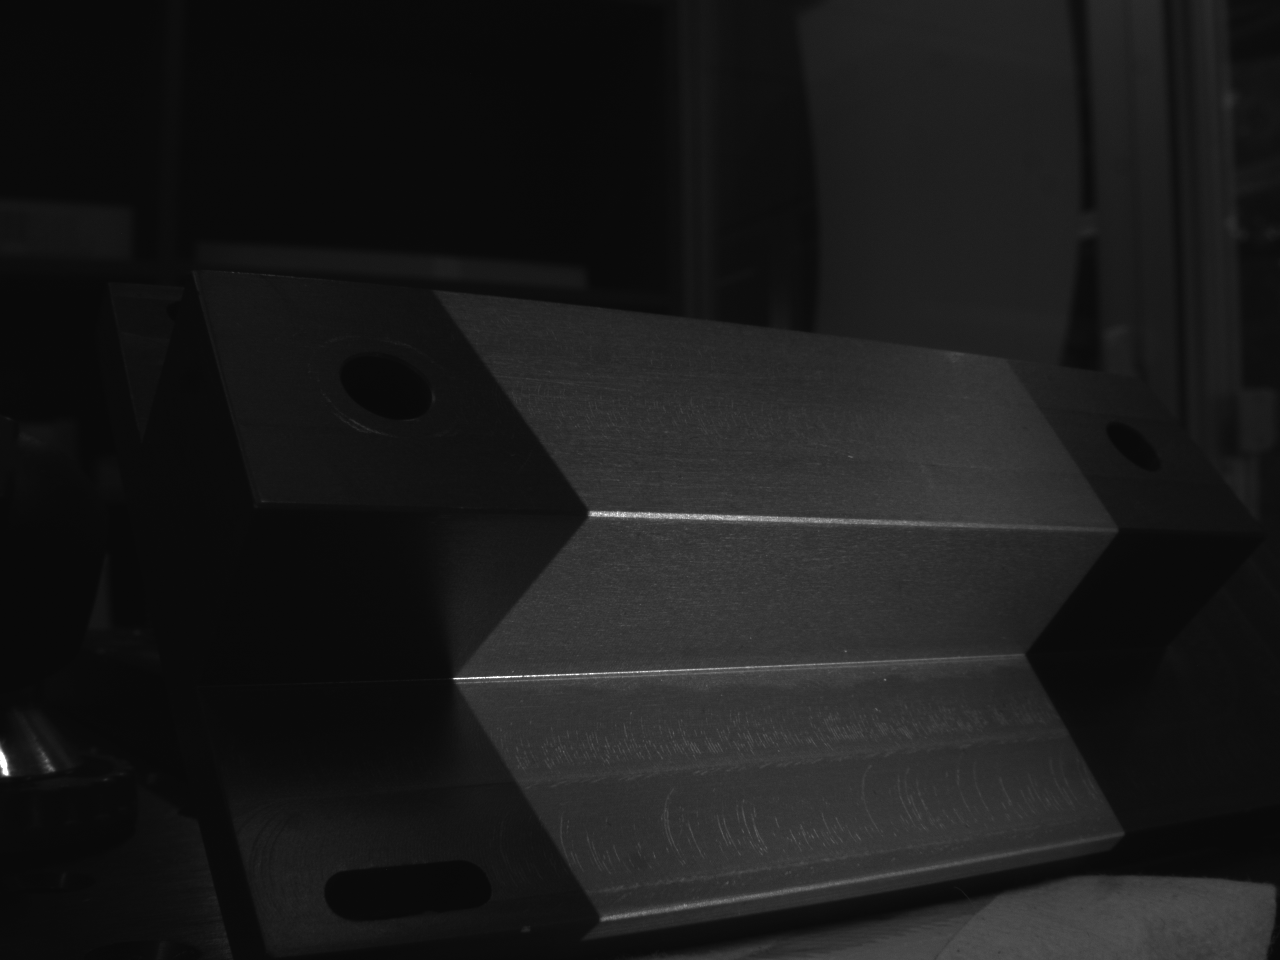
\includegraphics[width=0.49\linewidth]{images/snapshots_scan/SIMULATED-LEFT-LUMENERA-SN8010129/gray_08}
        }
        \subfloat{
            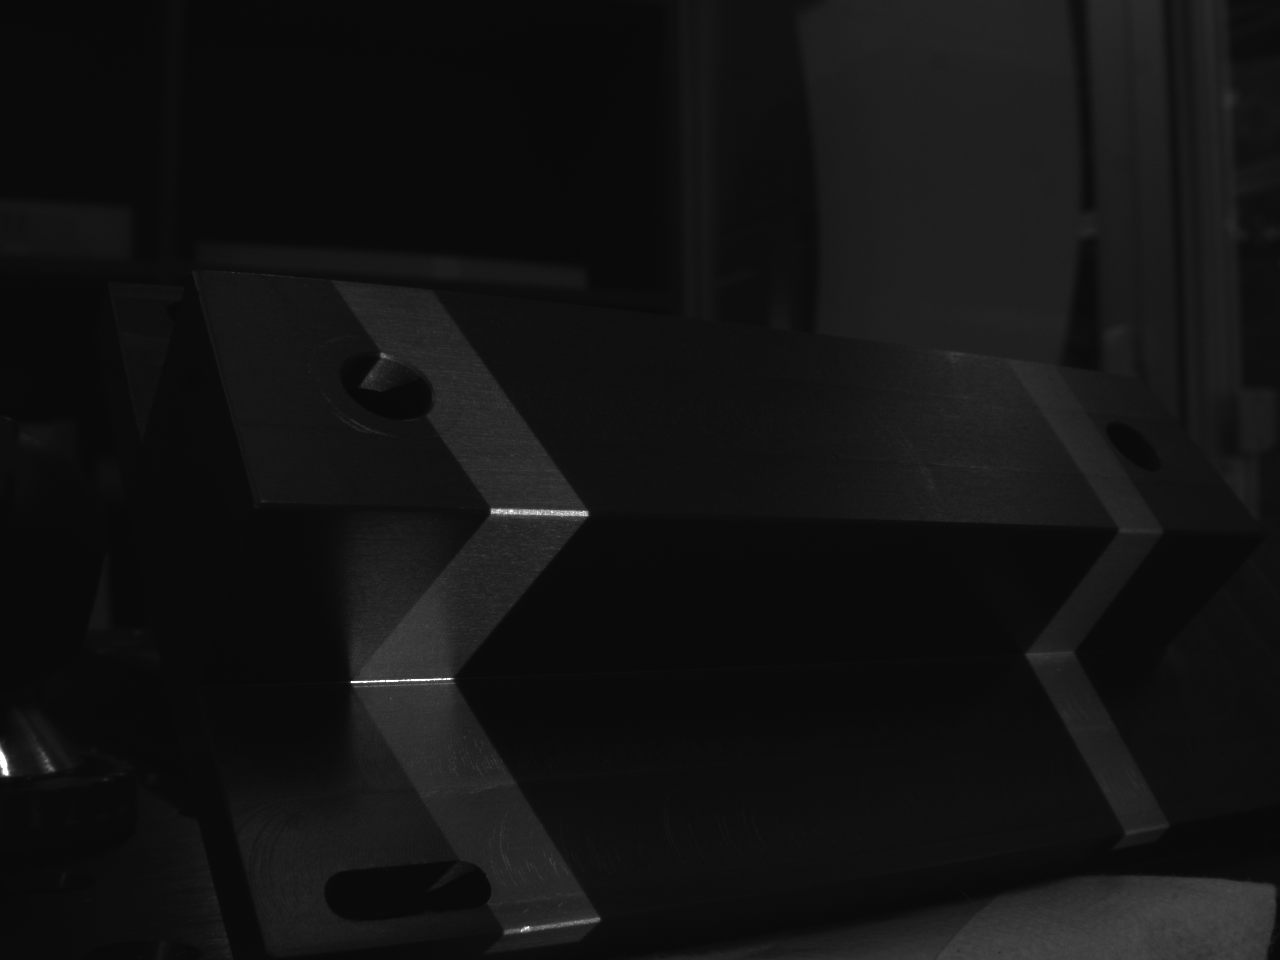
\includegraphics[width=0.49\linewidth]{images/snapshots_scan/SIMULATED-LEFT-LUMENERA-SN8010129/gray_08_inv}
        }
        \\
        \subfloat{
            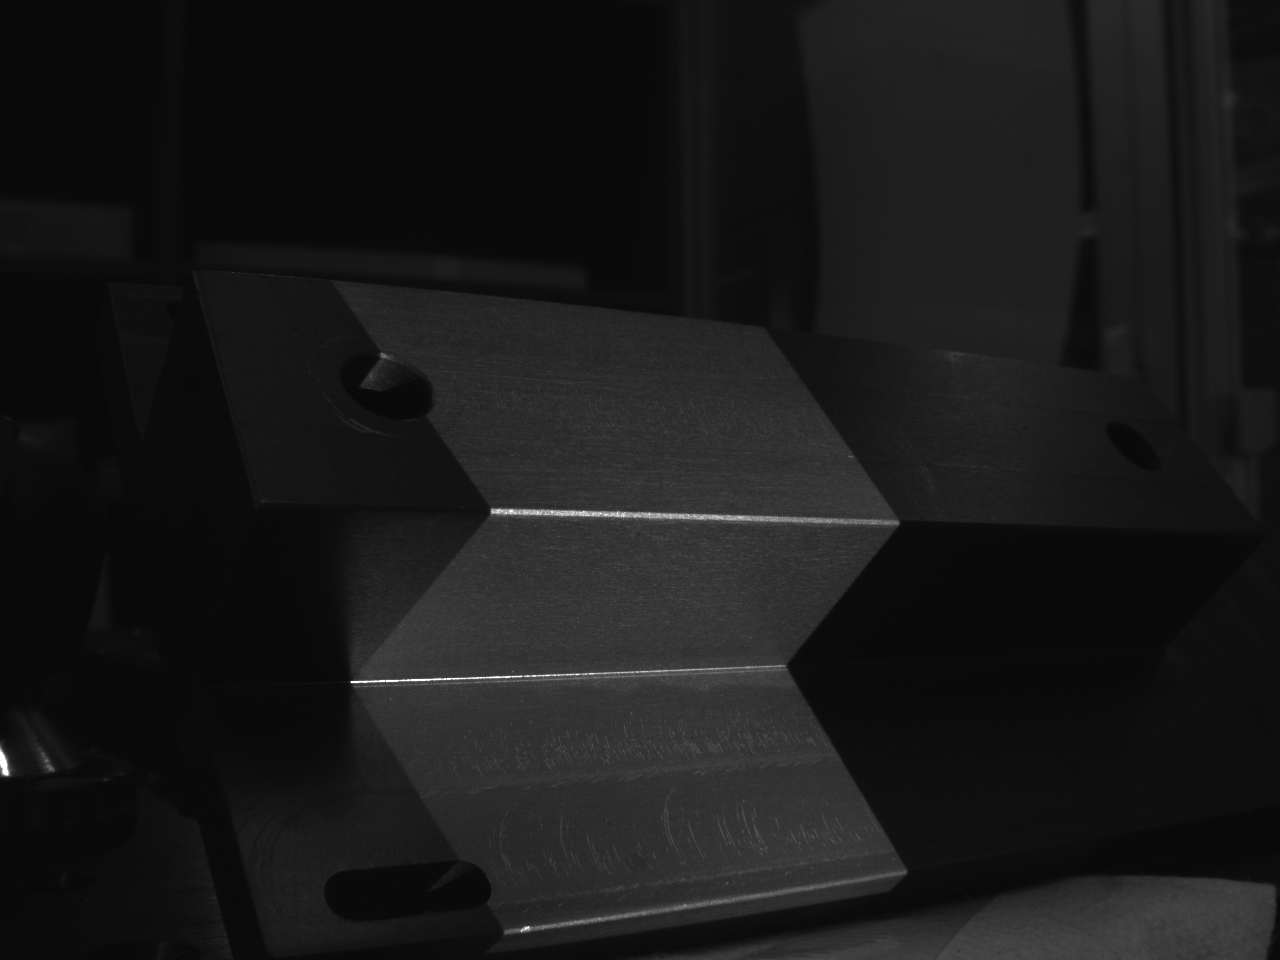
\includegraphics[width=0.49\linewidth]{images/snapshots_scan/SIMULATED-LEFT-LUMENERA-SN8010129/gray_09}
        }
        \subfloat{
            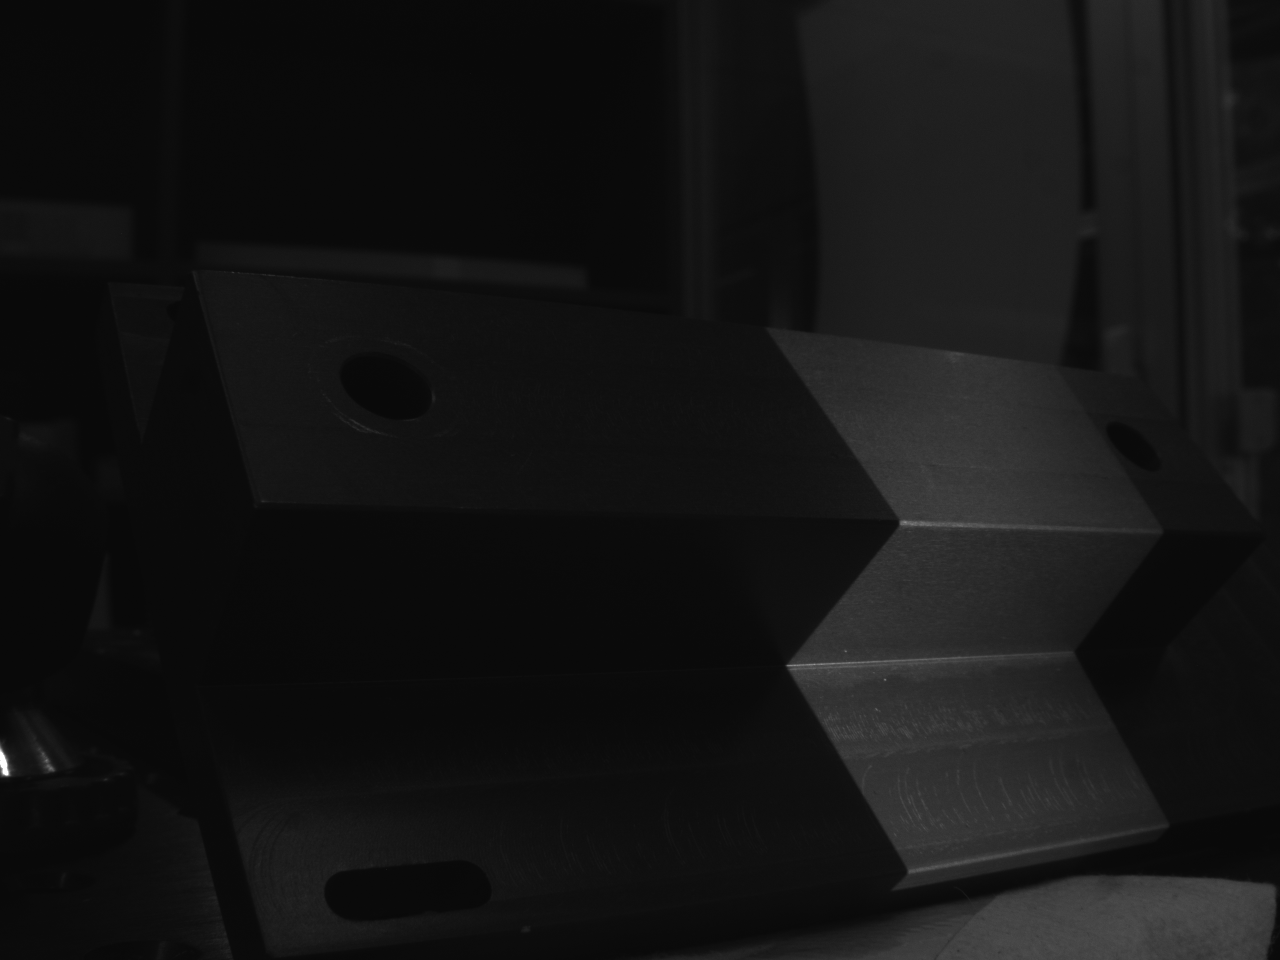
\includegraphics[width=0.49\linewidth]{images/snapshots_scan/SIMULATED-LEFT-LUMENERA-SN8010129/gray_09_inv}
        }
        \caption{Cámara izquierda: 5 últimos patrones proyectados (izq.) y su inverso (der.)}
        \label{fig:ejemploProyeccionCamaraIzquierda5a9}
\end{figure}

\begin{figure}[!bth]
    \myfloatalign
        \subfloat{
            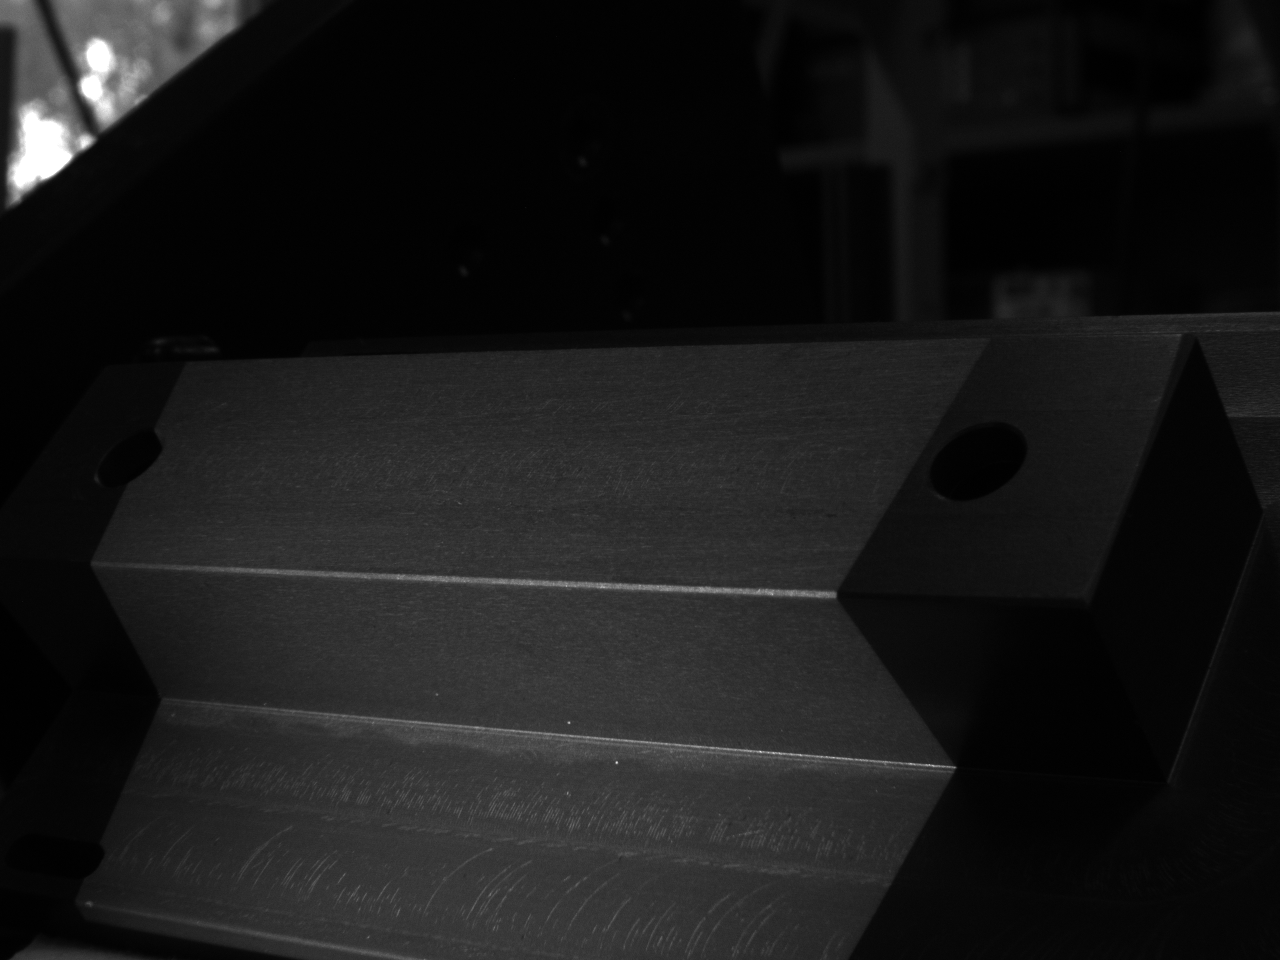
\includegraphics[width=0.49\linewidth]{images/snapshots_scan/SIMULATED-RIGHT-PGR-SN9041369/gray_00}
        }
        \subfloat{
            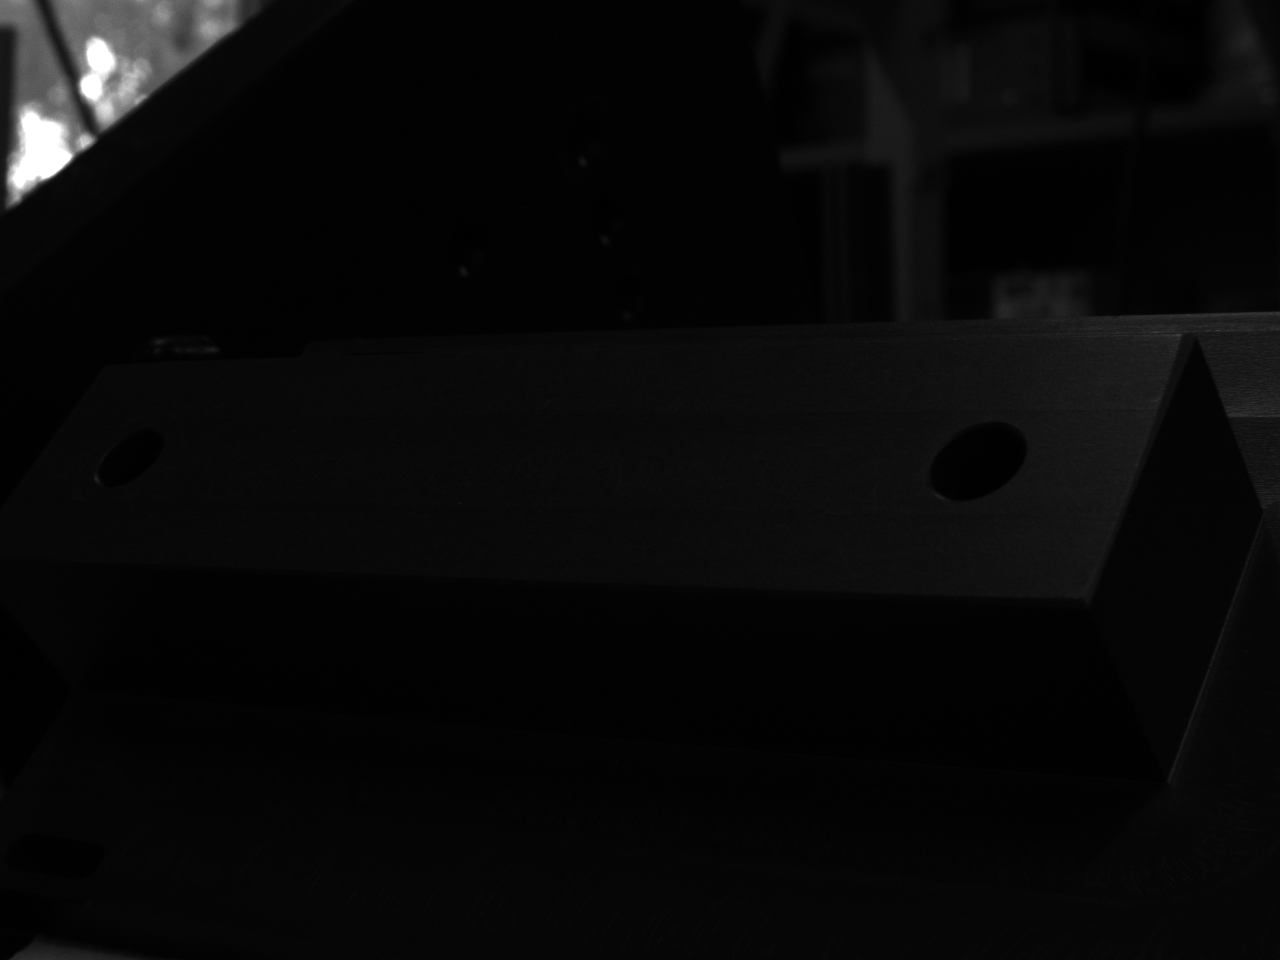
\includegraphics[width=0.49\linewidth]{images/snapshots_scan/SIMULATED-RIGHT-PGR-SN9041369/gray_00_inv}
        }
        \\
        \subfloat{
            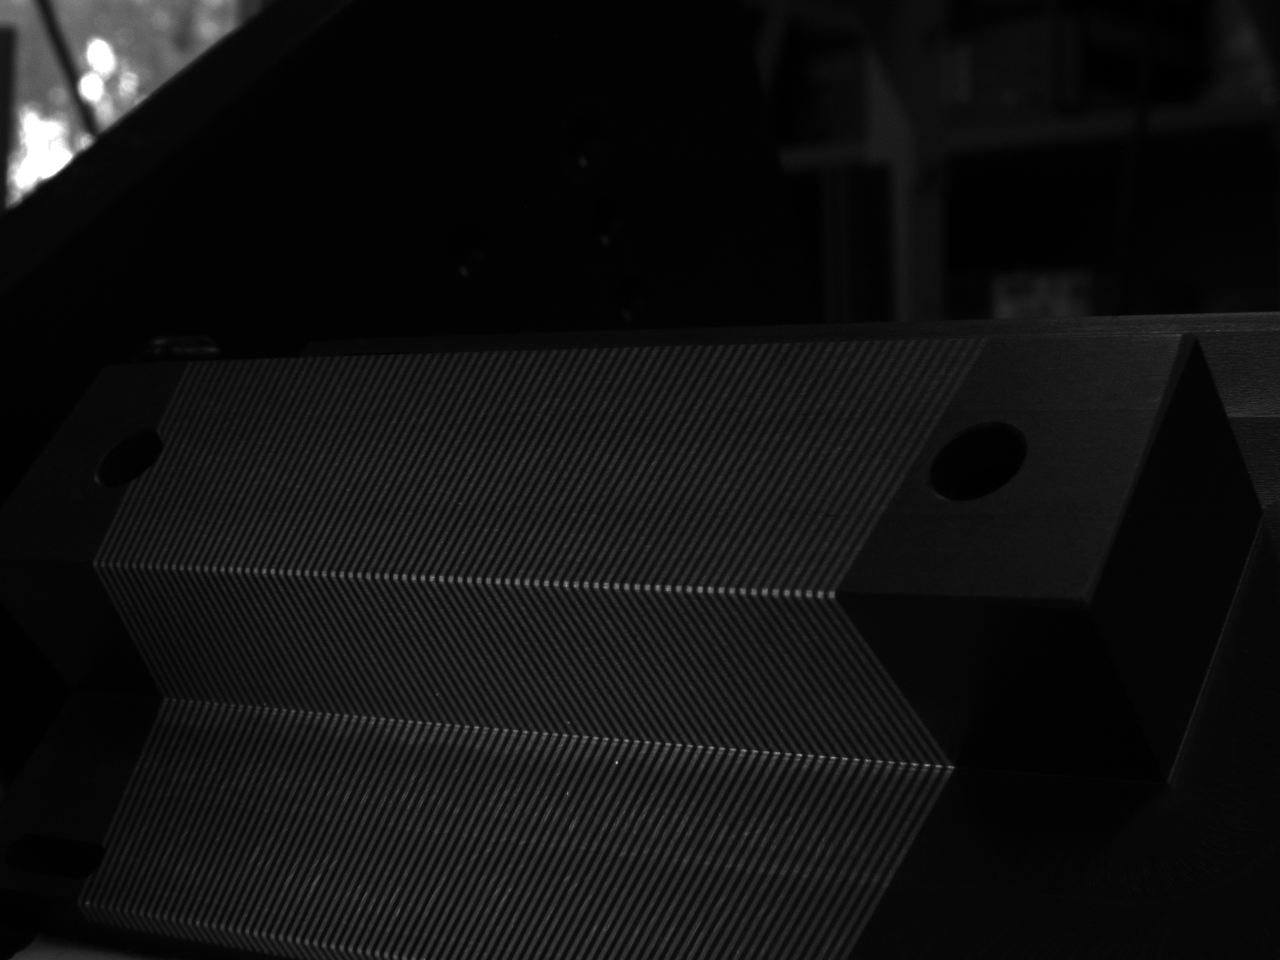
\includegraphics[width=0.49\linewidth]{images/snapshots_scan/SIMULATED-RIGHT-PGR-SN9041369/gray_01}
        }
        \subfloat{
            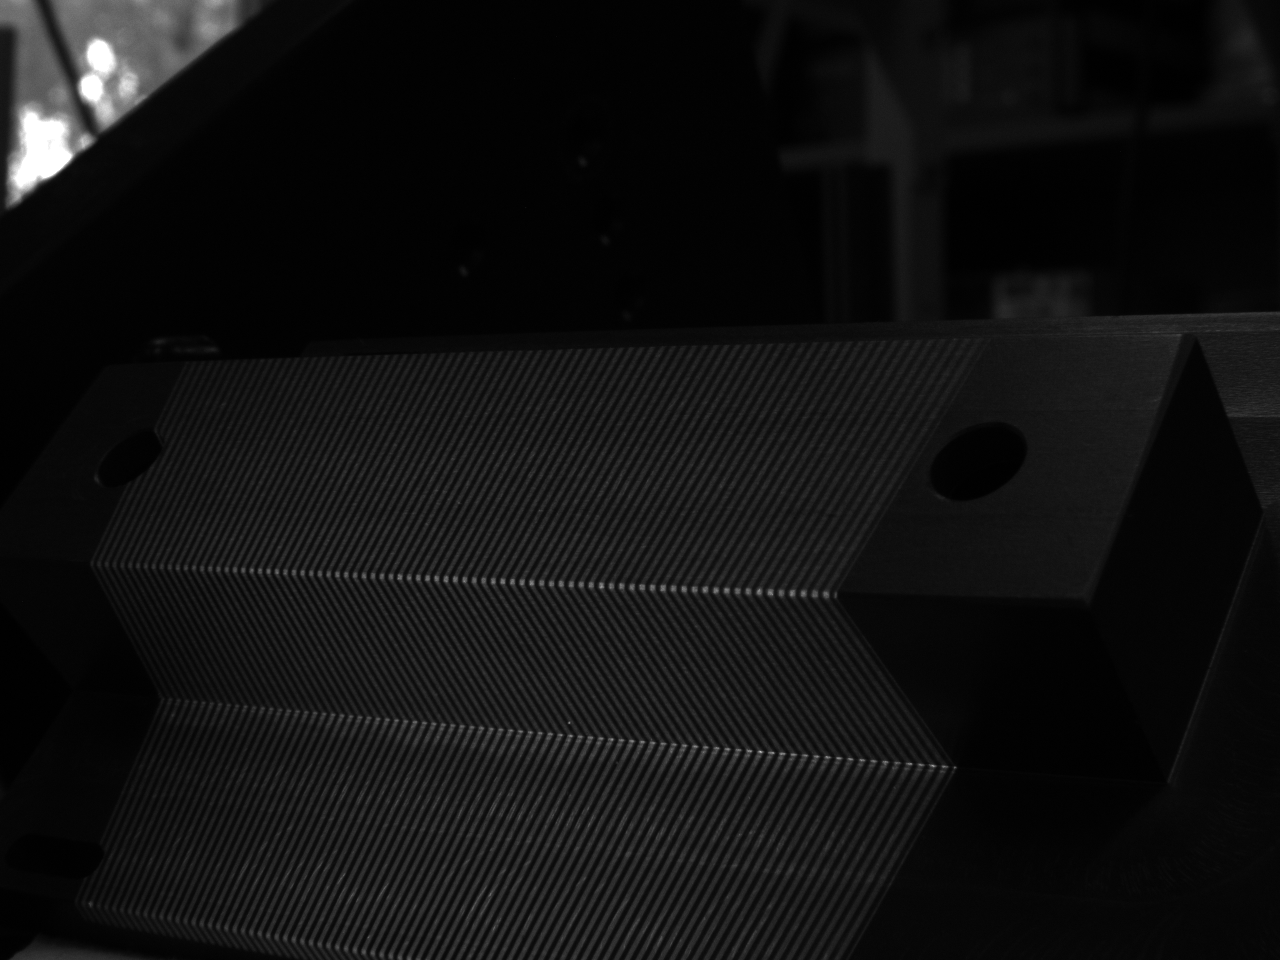
\includegraphics[width=0.49\linewidth]{images/snapshots_scan/SIMULATED-RIGHT-PGR-SN9041369/gray_01_inv}
        }
        \\
        \subfloat{
            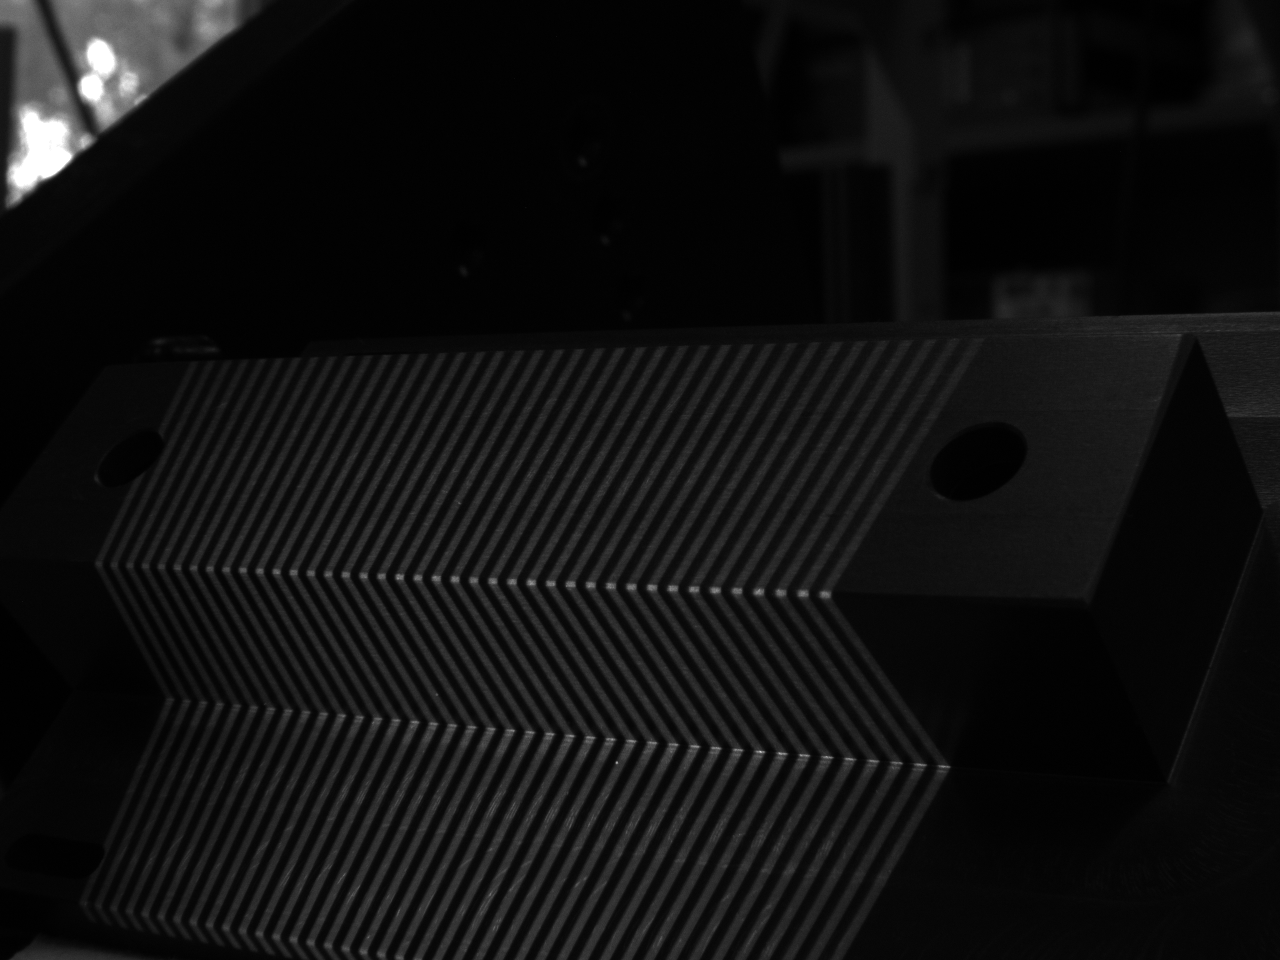
\includegraphics[width=0.49\linewidth]{images/snapshots_scan/SIMULATED-RIGHT-PGR-SN9041369/gray_02}
        }
        \subfloat{
            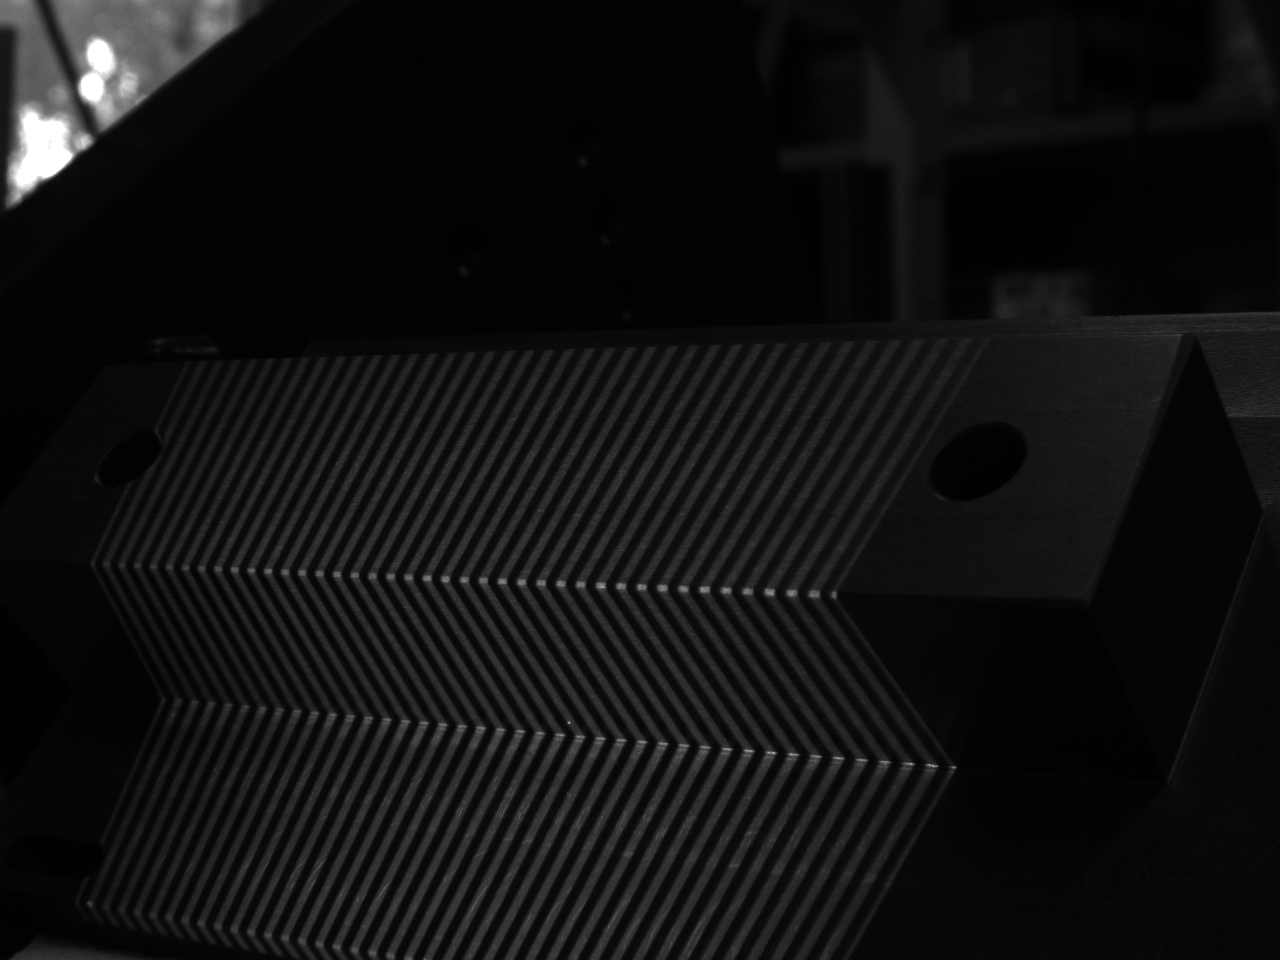
\includegraphics[width=0.49\linewidth]{images/snapshots_scan/SIMULATED-RIGHT-PGR-SN9041369/gray_02_inv}
        }
        \\
        \subfloat{
            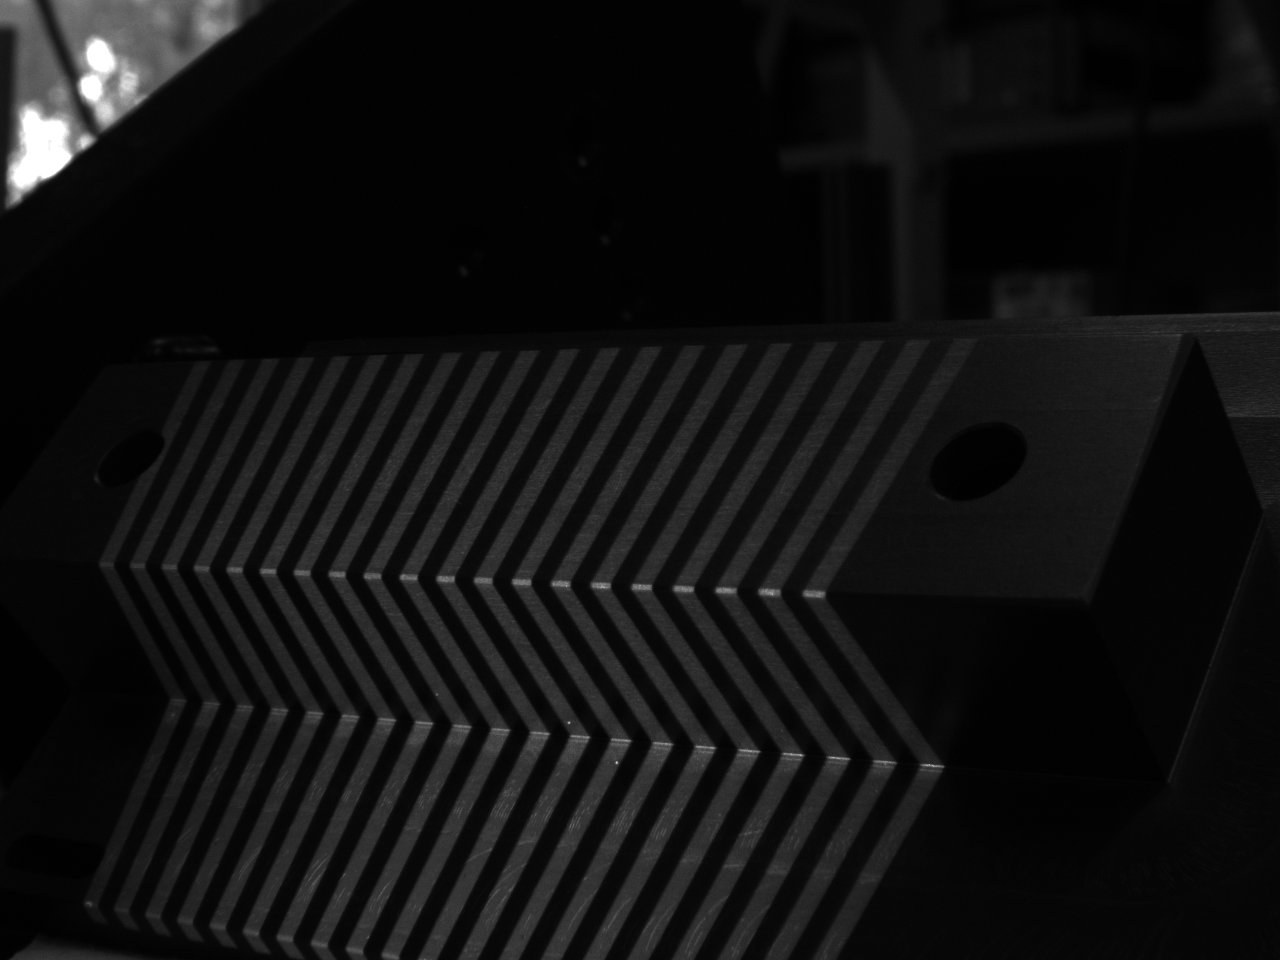
\includegraphics[width=0.49\linewidth]{images/snapshots_scan/SIMULATED-RIGHT-PGR-SN9041369/gray_03}
        }
        \subfloat{
            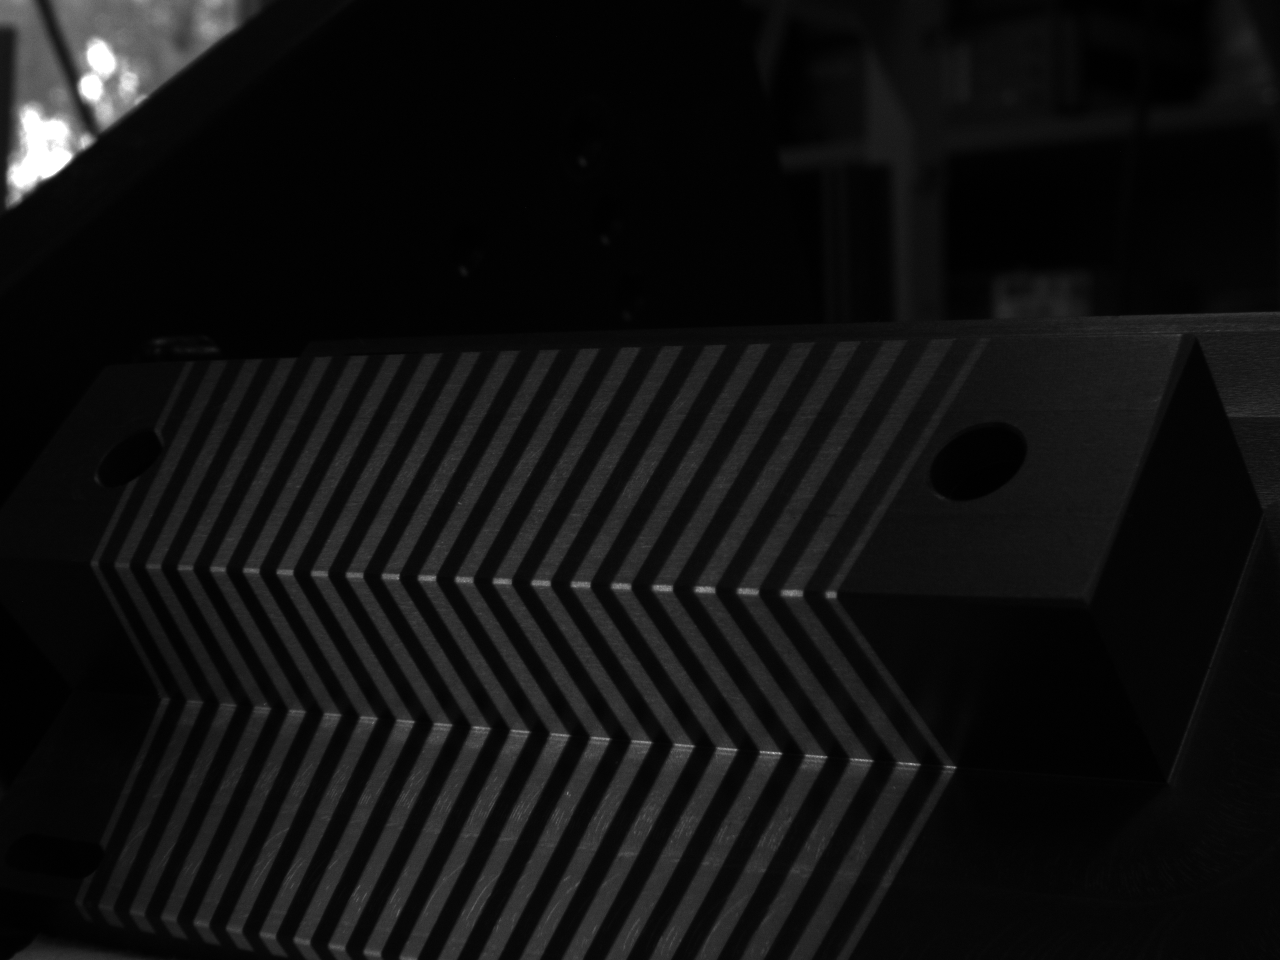
\includegraphics[width=0.49\linewidth]{images/snapshots_scan/SIMULATED-RIGHT-PGR-SN9041369/gray_03_inv}
        }
        \\
        \subfloat{
            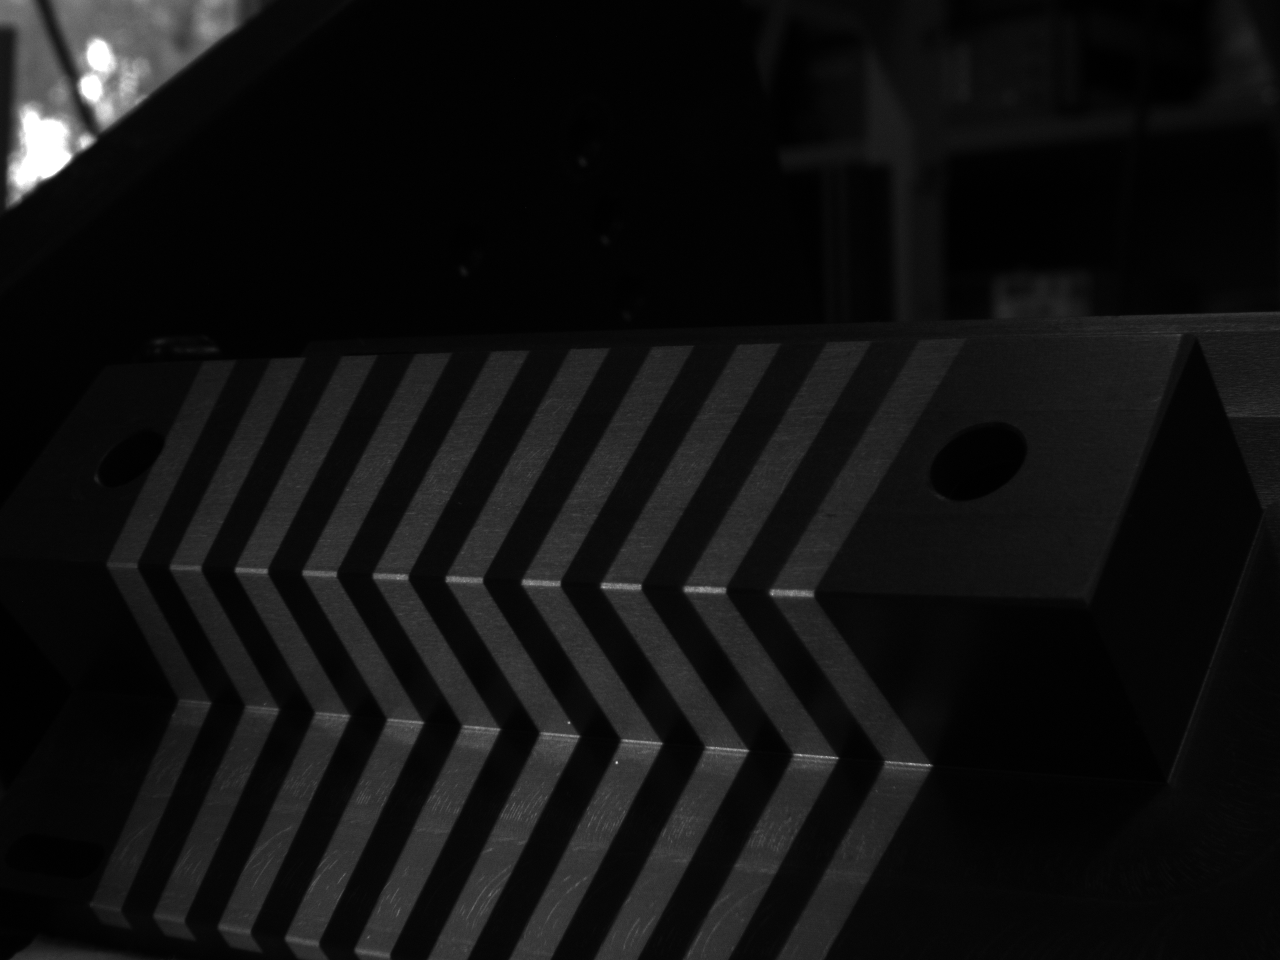
\includegraphics[width=0.49\linewidth]{images/snapshots_scan/SIMULATED-RIGHT-PGR-SN9041369/gray_04}
        }
        \subfloat{
            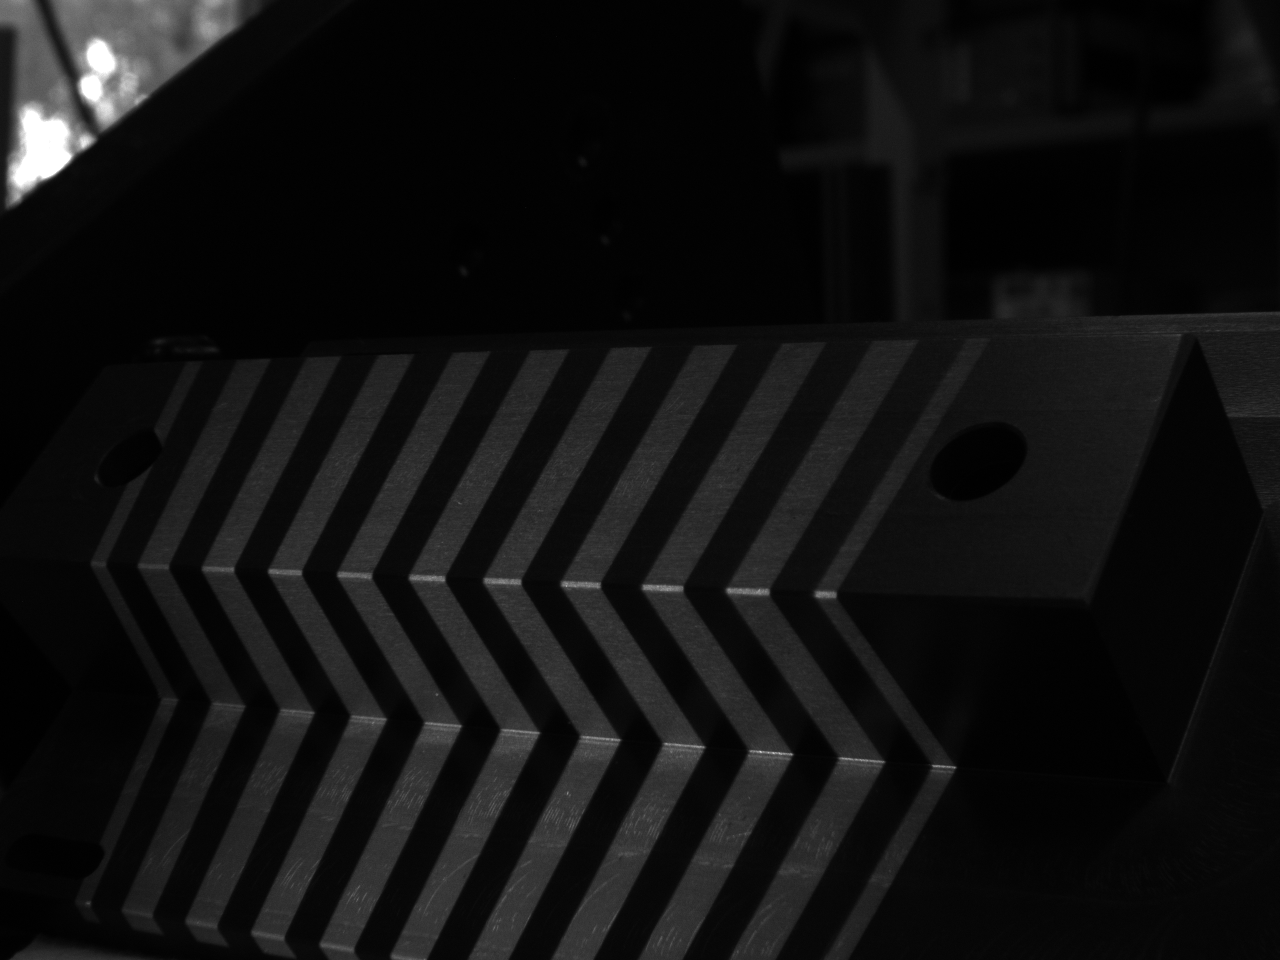
\includegraphics[width=0.49\linewidth]{images/snapshots_scan/SIMULATED-RIGHT-PGR-SN9041369/gray_04_inv}
        }
        \caption{Cámara derecha: 5 primeros patrones proyectados (izq.) y su inverso (der.)}
        \label{fig:ejemploProyeccionCamaraDerecha0a4}
\end{figure}

\begin{figure}[!bth]
    \myfloatalign
        \subfloat{
            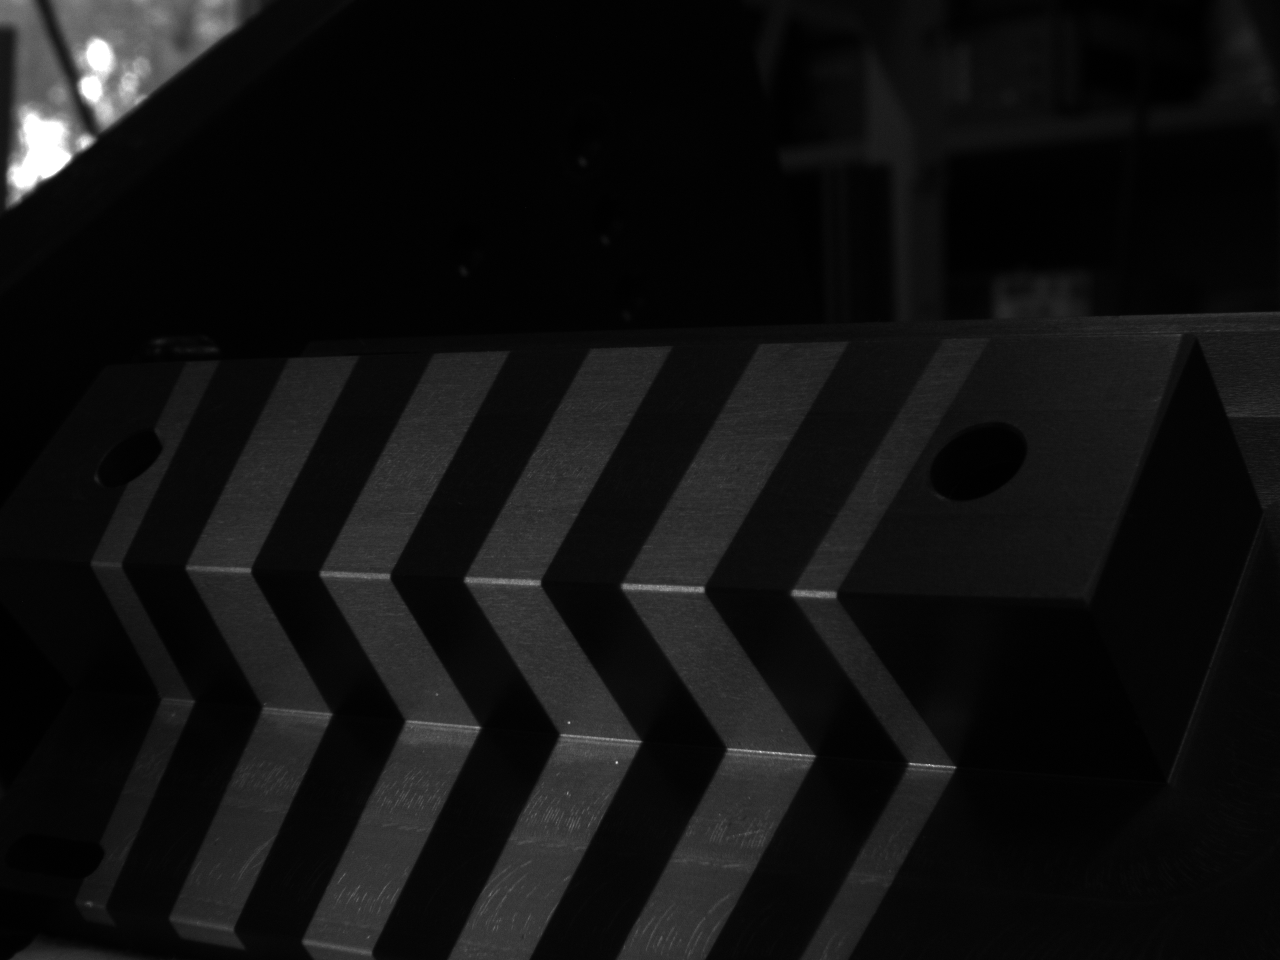
\includegraphics[width=0.49\linewidth]{images/snapshots_scan/SIMULATED-RIGHT-PGR-SN9041369/gray_05}
        }
        \subfloat{
            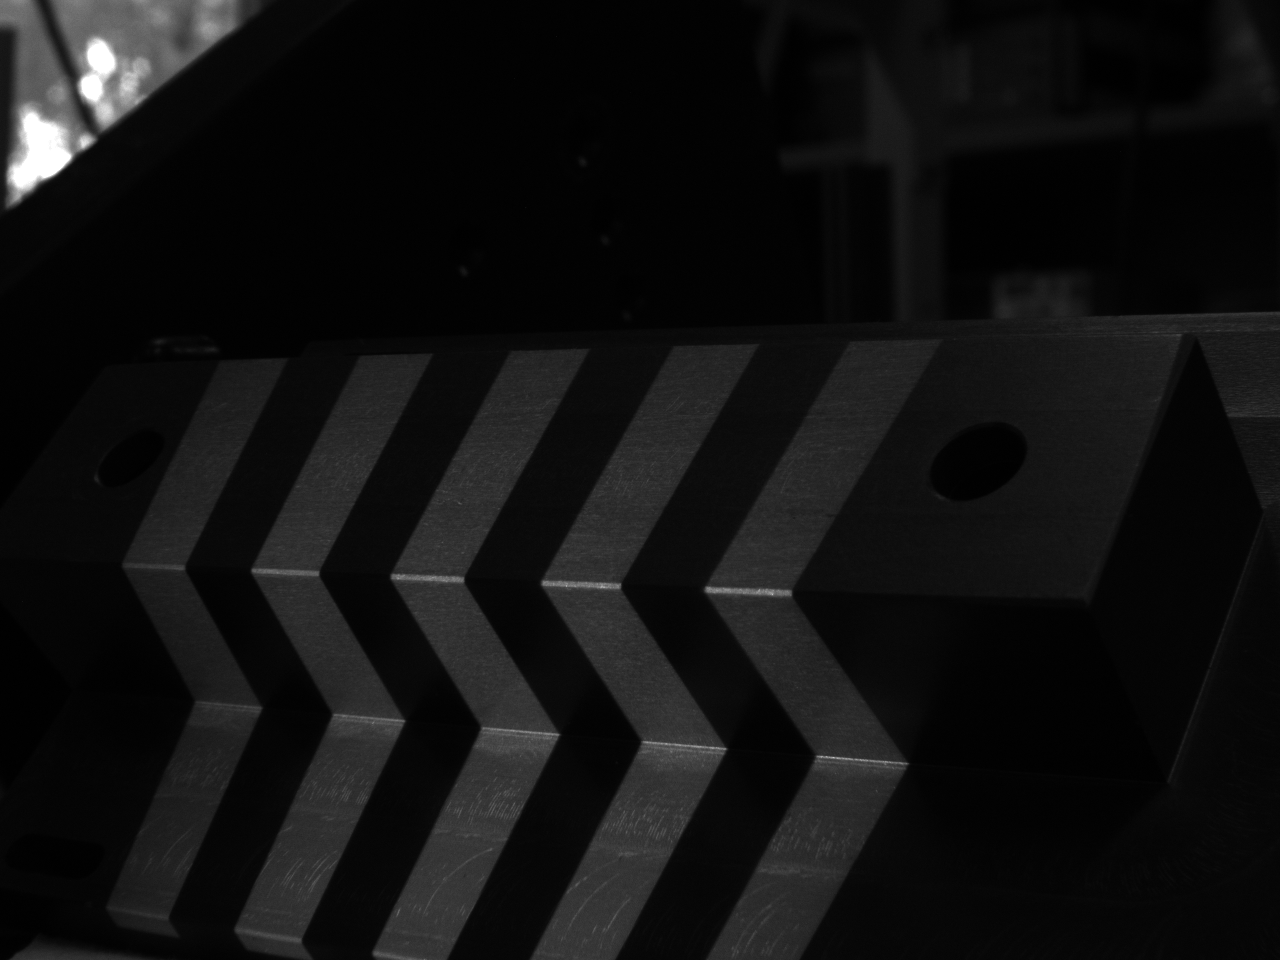
\includegraphics[width=0.49\linewidth]{images/snapshots_scan/SIMULATED-RIGHT-PGR-SN9041369/gray_05_inv}
        }
        \\
        \subfloat{
            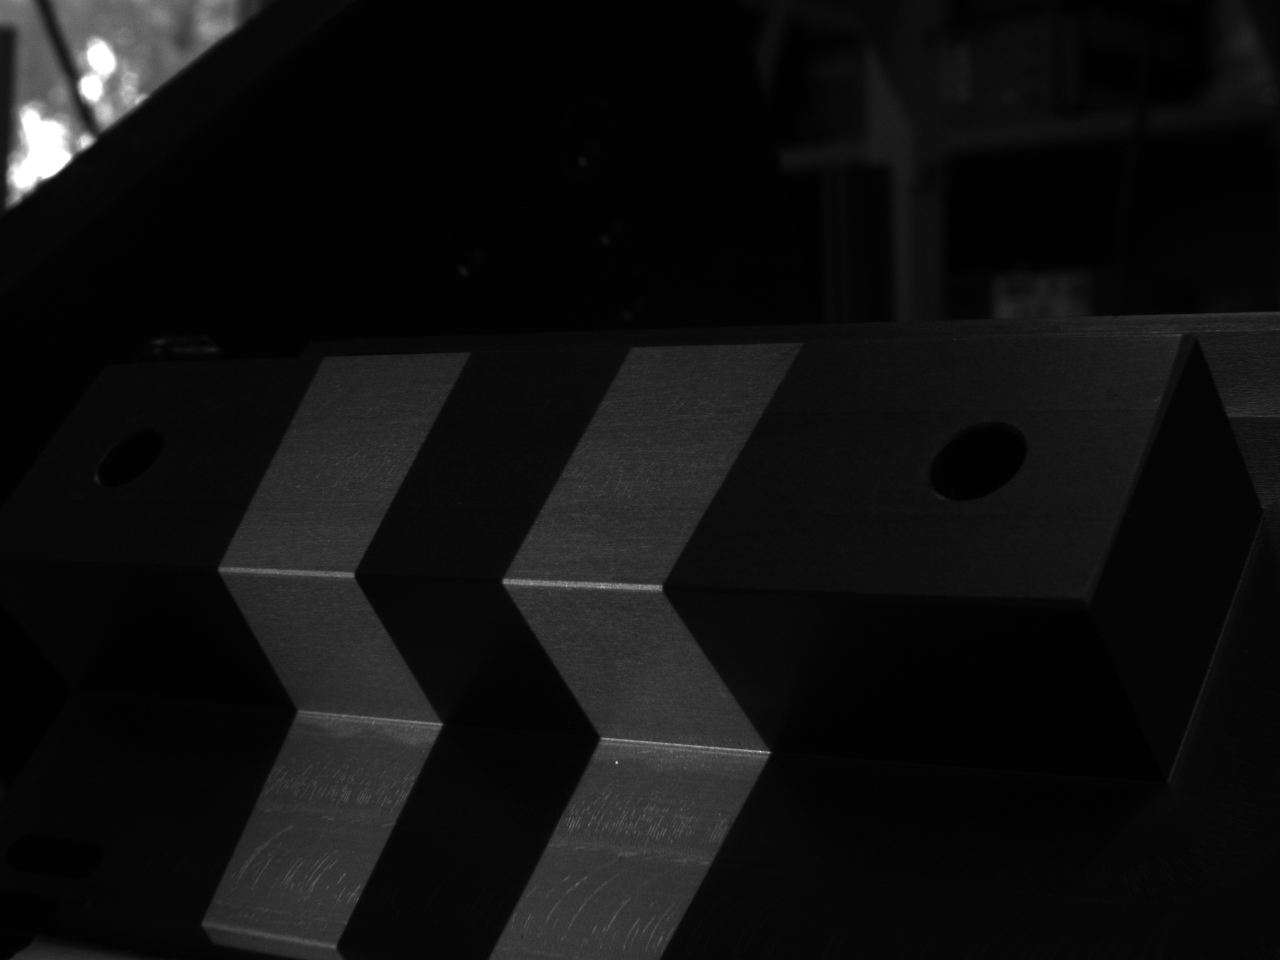
\includegraphics[width=0.49\linewidth]{images/snapshots_scan/SIMULATED-RIGHT-PGR-SN9041369/gray_06}
        }
        \subfloat{
            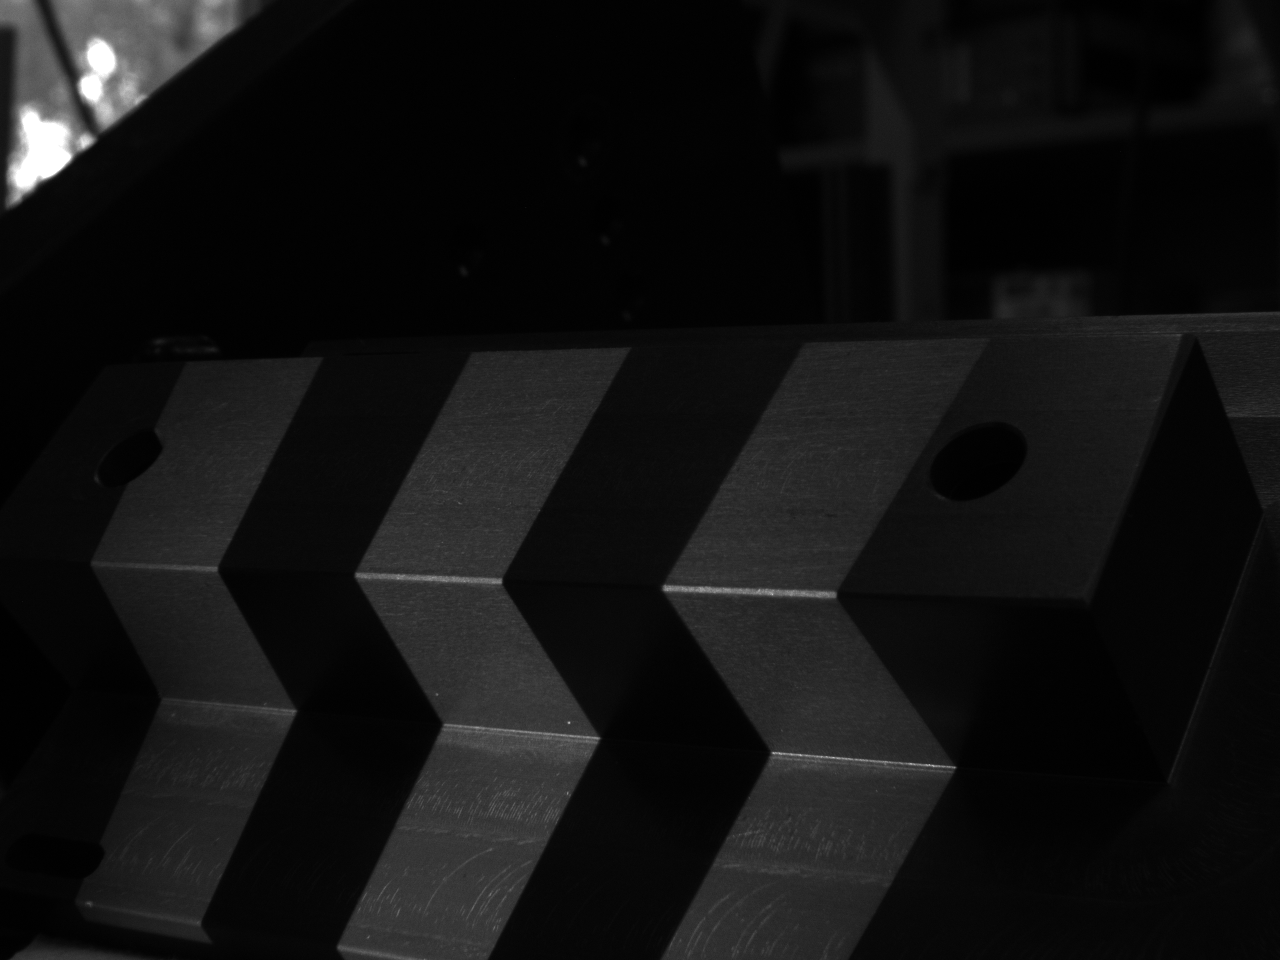
\includegraphics[width=0.49\linewidth]{images/snapshots_scan/SIMULATED-RIGHT-PGR-SN9041369/gray_06_inv}
        }
        \\
        \subfloat{
            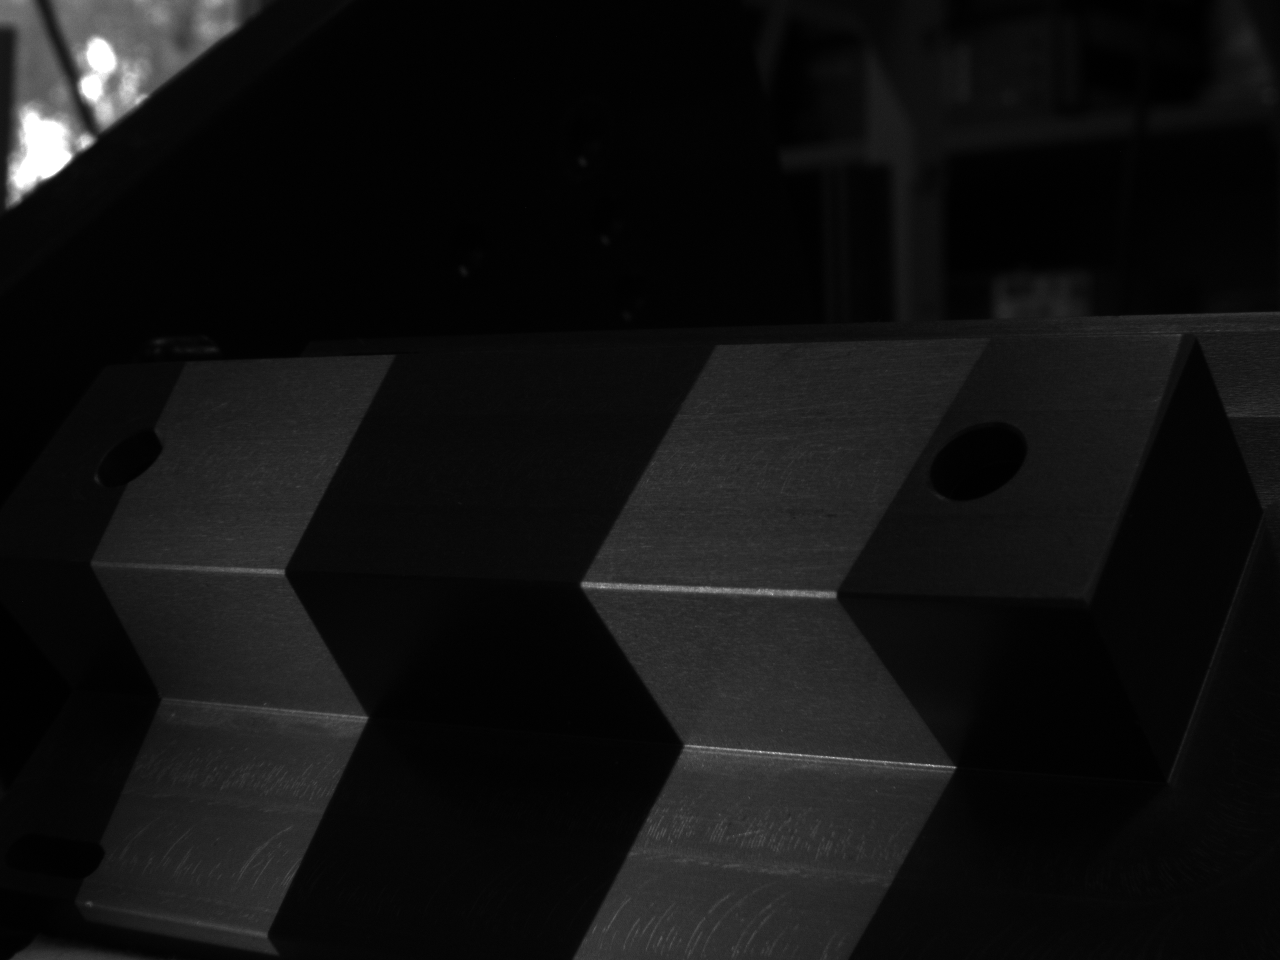
\includegraphics[width=0.49\linewidth]{images/snapshots_scan/SIMULATED-RIGHT-PGR-SN9041369/gray_07}
        }
        \subfloat{
            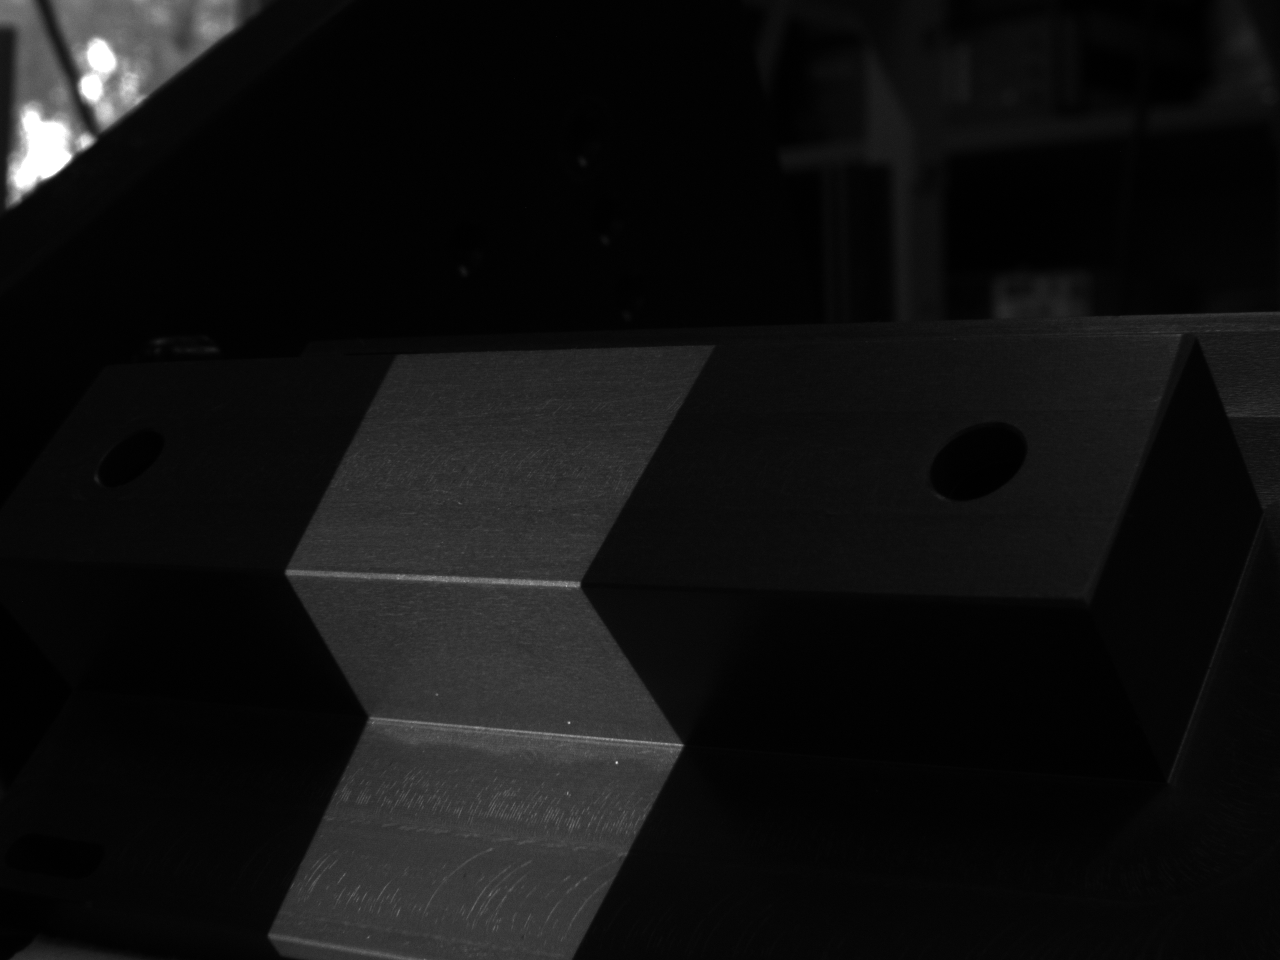
\includegraphics[width=0.49\linewidth]{images/snapshots_scan/SIMULATED-RIGHT-PGR-SN9041369/gray_07_inv}
        }
        \\
        \subfloat{
            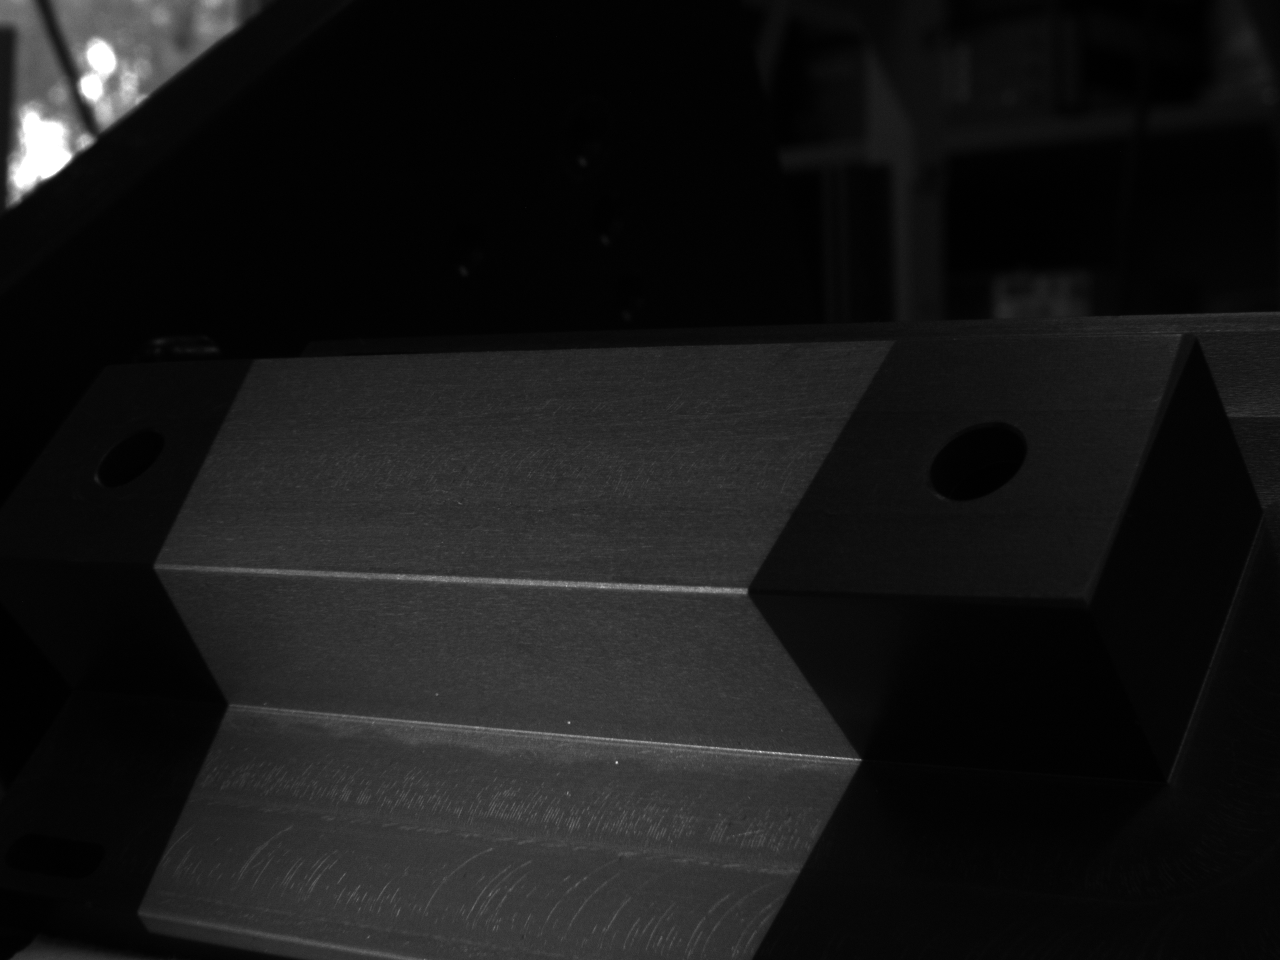
\includegraphics[width=0.49\linewidth]{images/snapshots_scan/SIMULATED-RIGHT-PGR-SN9041369/gray_08}
        }
        \subfloat{
            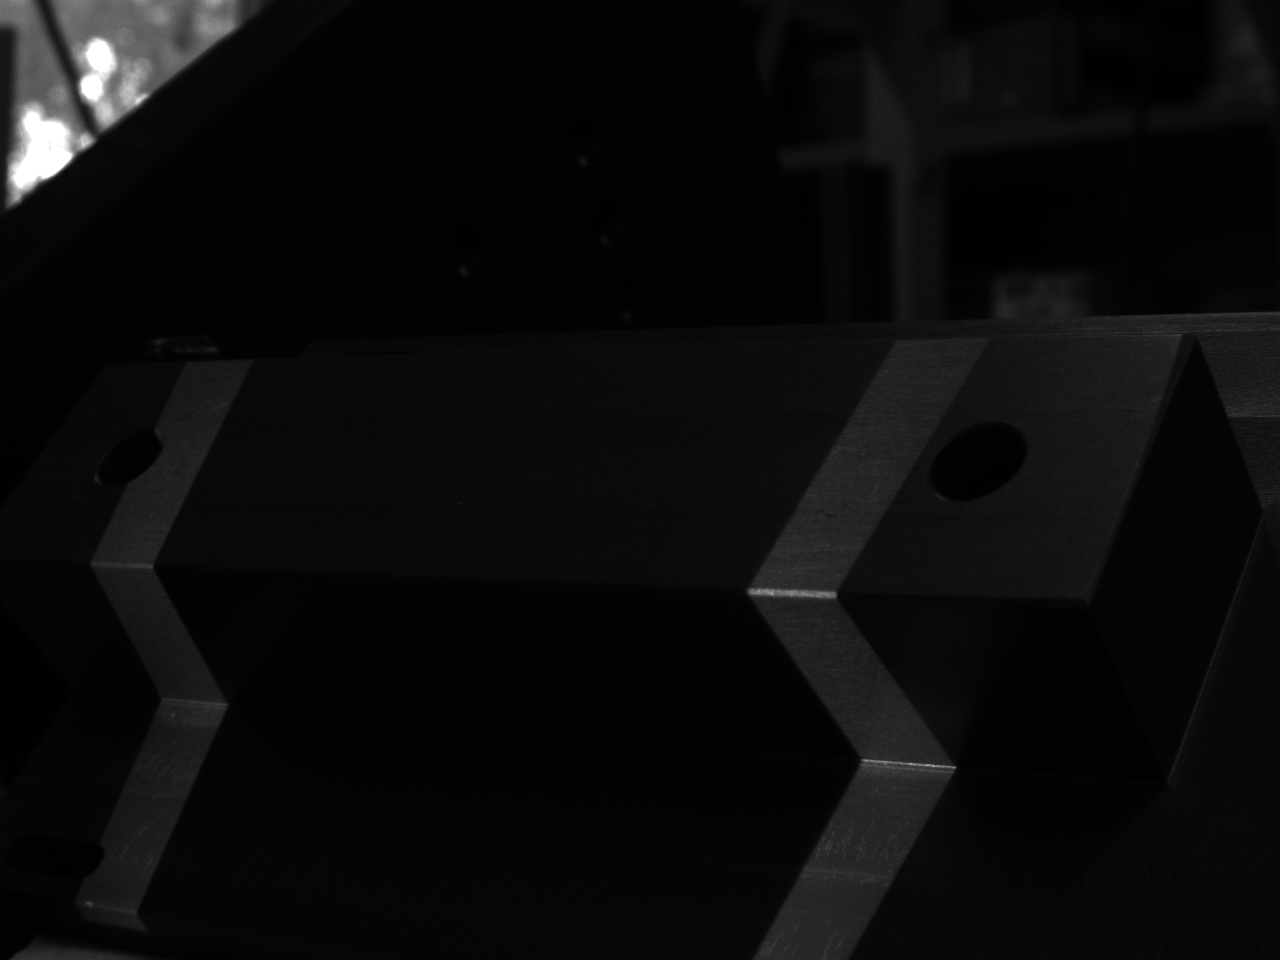
\includegraphics[width=0.49\linewidth]{images/snapshots_scan/SIMULATED-RIGHT-PGR-SN9041369/gray_08_inv}
        }
        \\
        \subfloat{
            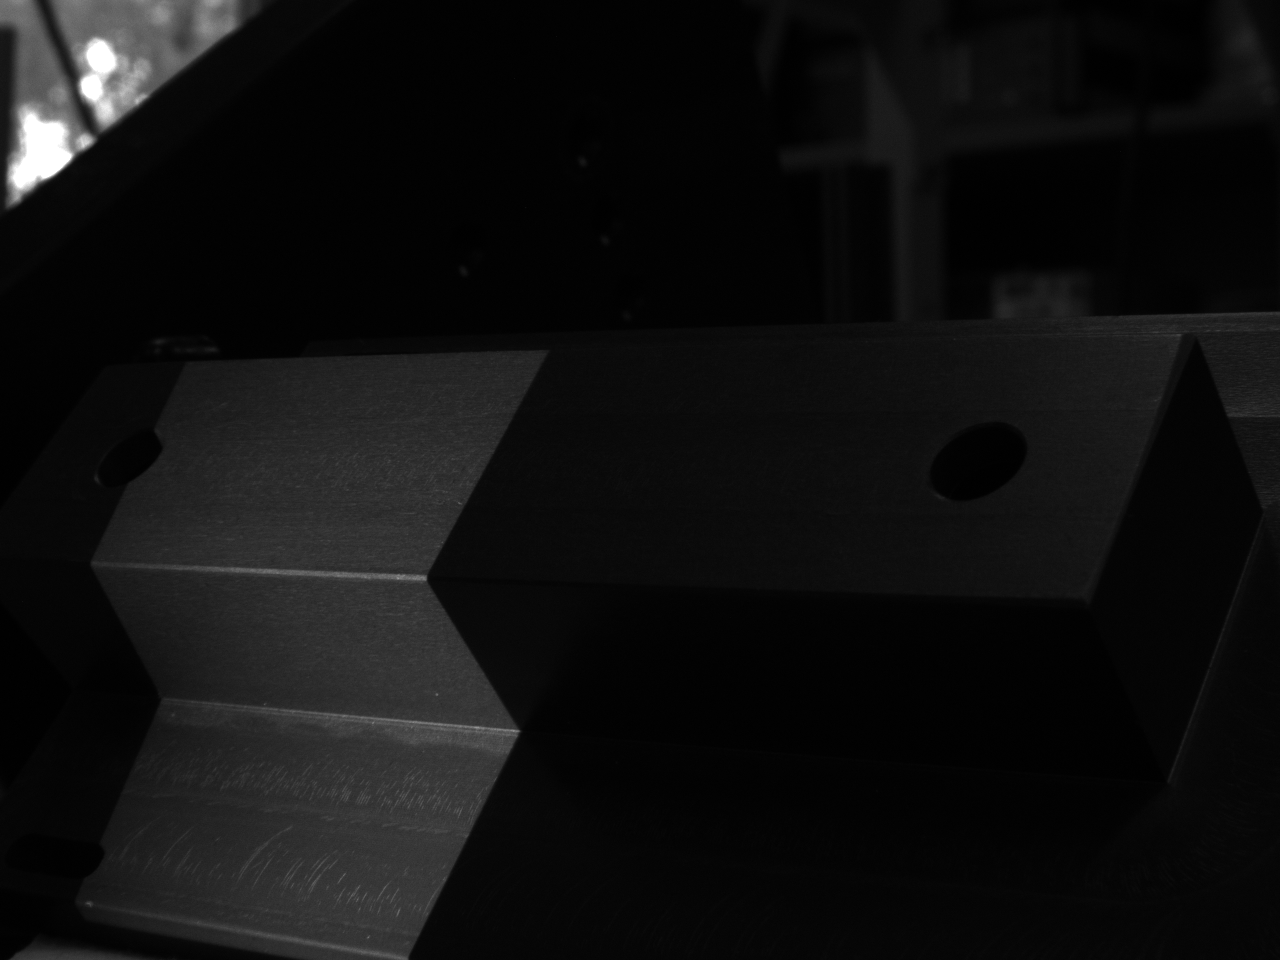
\includegraphics[width=0.49\linewidth]{images/snapshots_scan/SIMULATED-RIGHT-PGR-SN9041369/gray_09}
        }
        \subfloat{
            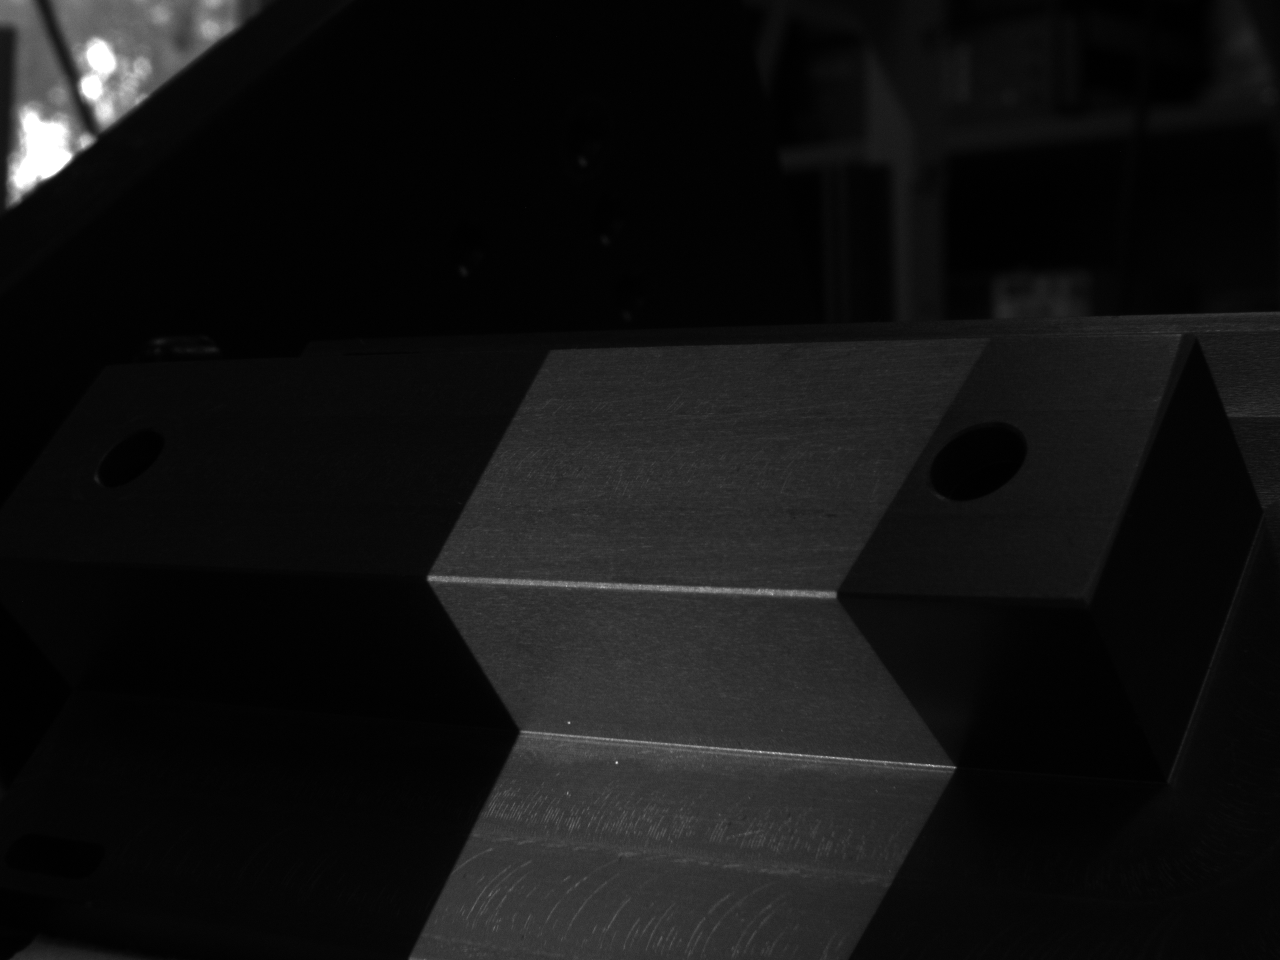
\includegraphics[width=0.49\linewidth]{images/snapshots_scan/SIMULATED-RIGHT-PGR-SN9041369/gray_09_inv}
        }
        \caption{Cámara derecha: 5 últimos patrones proyectados (izq.) y su inverso (der.)}
        \label{fig:ejemploProyeccionCamaraDerecha5a9}
\end{figure}
